\documentclass[11pt]{article}

% ============================================================
% PACKAGES
% ============================================================

\usepackage[T1]{fontenc}
\usepackage{microtype}

\usepackage{graphicx}
\usepackage{caption}
\usepackage{subcaption}
\graphicspath{{documentation/resources/mqa-designs/}{plots/}{plots_prefill_corrected/}{images/}{./}}

\usepackage[style=apa]{biblatex}
\addbibresource{bib.bib}

\usepackage{geometry}
\usepackage{amsmath}
\usepackage{amssymb}
\usepackage{booktabs}
\usepackage{enumitem}
\usepackage{float}
\usepackage[hidelinks]{hyperref}

% ============================================================
% FORMATTING
% ============================================================

\geometry{
    a4paper,
    total={170mm,257mm},
    left=20mm,
    top=20mm,
}

\setlength{\parindent}{0pt}
\setlength{\parskip}{0.45em}

\linespread{1.03}

% ============================================================
% TITLE
% ============================================================

\title{
\textbf{
Performance Modeling of a Key-Value-Stationary
Systolic Array for Multi-Query Attention Inference
}
\\[1ex]
\large Mid-Progress Report
}

\author{
Hudson Strauss \and Dhruv Patel
}

\date{\today}

% ============================================================
% DOCUMENT
% ============================================================

\begin{document}

\maketitle

\begin{center}
High-Performance Computer Architecture and Systems \\
Santa Clara University
\end{center}

\vspace{0.5em}

% ============================================================
\section{Introduction}

Transformer inference has made memory-efficient attention a central
systems problem. During autoregressive decoding, each generated token
repeatedly accesses the key-value (KV) cache, causing memory traffic
to scale with sequence length. As context windows increase, inference
becomes increasingly memory-bound rather than compute-bound.

Multi-Query Attention (MQA) reduces this overhead by sharing keys and
values across multiple query heads, substantially lowering KV-cache
footprint compared to standard multi-head attention
\parencite{ainslie2023gqa}. However, most accelerators still map
attention onto generic matrix multiplication hardware despite the
streaming nature of autoregressive decoding.

Traditional systolic-array dataflows --- output-stationary,
weight-stationary, and input-stationary --- are optimized for
dense GEMM workloads and do not exploit the fact that during
MQA inference, queries stream continuously while keys and
values remain relatively fixed across heads.

This report presents an analytical performance model of a
KV-stationary systolic-array mapping for MQA inference,
validated against SCALE-Sim cycle-accurate simulation.
We sweep sequence length, merge-extension depth, and
interleaved-MAC count, comparing the architecture against
both a roofline baseline and a FlashAttention-style fused
reference on equal silicon.
The key finding is that the architecture delivers a genuine
\(\sim\)1.75$\times$ area-normalized throughput advantage
over FlashAttention at prefill for sequences up to
\(T = 2{,}048\) (SCALE-Sim validated).
Autoregressive decode is not validated in this work;
the analytical model projects significant DRAM savings
from holding the KV cache on-chip, and a two-pass decode
extension is identified as the primary path to reducing
chip area for practical deployment.

% ============================================================
\section{Problem Statement}

The goal of this project is to evaluate a KV-stationary systolic-array
dataflow for MQA inference and determine the conditions under which
it outperforms conventional systolic mappings.

For each incoming query vector \(Q\), attention decoding proceeds
in three stages:

\vspace{-0.5em}

\[
s_i = Q \cdot K_i
\]

\[
a_i =
\frac{e^{s_i}}
{\sum_j e^{s_j}}
\]

\[
O = \sum_i a_i V_i
\]

\vspace{-0.5em}

where:

\begin{center}
\begin{tabular}{ll}
\(Q\) & Incoming query vector \\
\(K_i\) & Key stored in PE column \(i\) \\
\(V_i\) & Value vector stored in PE column \(i\) \\
\(s_i\) & Local attention score \\
\(a_i\) & Normalized attention weight \\
\end{tabular}
\end{center}

A critical bottleneck in conventional hardware is the
softmax normalization step: computing
\(\sum_j e^{s_j}\) requires a complete pass over all scores,
forcing either (a) the full \(T \times T\) score matrix to be
materialized in DRAM before normalization, or (b) a two-pass
on-chip tiling strategy as in FlashAttention.
At \(T = 8{,}192\) with \(H = 64\) heads, materializing scores
requires writing and re-reading \textbf{16\,GB} of intermediate
data per prefill pass.

The proposed architecture resolves this by computing the
online softmax update inline at each PE column, eliminating
the score matrix entirely.

% ============================================================
\section{Proposed Architecture}

\subsection{Design Evolution}

The architecture went through four distinct iterations before
arriving at the final configuration.
Each iteration was motivated by a measurable inefficiency in
the previous design.

\textbf{Iteration 1 --- Basic 1D KV-stationary pipeline.}
The starting point is a single row of processing elements,
each storing one \((K_i, V_i)\) pair.
A query vector enters at column~0 and streams left-to-right,
computing a running attention score at each column using the
online softmax update described in \S2.
This eliminates score-matrix DRAM traffic but immediately
exposes a pipeline drain problem: after the query packet enters
the last column it must still traverse all remaining
\(\text{cols} - 1\) columns before the result is available.
At \(T = 8{,}192\) with no partitioning, drain accounts for
essentially 100\% of total latency.
A second problem is also present but less obvious at this stage:
the dot product in each column takes \(d = 128\) cycles,
while the upper Running Attention PE needs only 7 cycles to
process the resulting score.
The upper PE therefore sits idle for 121 of every 135 column
cycles --- a utilization of \(\approx\)5\%.

\textbf{Iteration 2 --- 2D multi-head extension.}
The natural extension is to assign each of the \(H = 64\)
query heads its own row lane.
MQA's defining property --- all heads share a single K and V
cache --- means the same column data is broadcast vertically
to all rows simultaneously.
KV is loaded once from DRAM regardless of head count.
This fills the Y-axis of the array and improves total throughput
\(H\times\), but does not address the drain problem or the
5\% upper PE utilization.

\textbf{Iteration 3 --- Merge extensions to reduce drain overhead.}
To reduce drain, the sequence is partitioned across \(2^n\)
parallel sub-arrays.
Each sub-array handles \(T / 2^n\) tokens, so drain shrinks
from \(T - 1\) to \(T / 2^n - 1\) pipeline steps.
A binary tree of inline merge PEs (Figure~\ref{fig:merge_reduction})
combines the partial \((m, l, O)\) softmax states from each
sub-array in \(n\) reduction levels, producing the correct
normalised output with no post-pipeline overhead.
With \(n = 3\): drain drops \(8\times\) at the cost of
\(8\times\) more PE rows.
This produced a validated speedup but an area-normalized
efficiency of only 1.29$\times$ over FlashAttention at
\(T = 8{,}192\) --- the extra rows are expensive relative
to the gain.

\textbf{Iteration 4 --- Interleaved MACs (\(lmc\)) to improve PE utilization.}
Profiling the cycle breakdown revealed that merge extensions
were treating the symptom (drain) rather than the root cause
(idle upper PEs).
With a single MAC per column the upper PE fires once every
135 cycles but needs only 7 --- a 95\% idle rate.
The fix is to time-interleave \(lmc\) independent MAC units
within each column, each servicing a different query packet
offset by \(\lceil d / lmc \rceil\) cycles.
With \(lmc = 16\): a new query packet starts every 8 cycles
instead of every 128, and upper PE utilization rises from
5\% to 87.5\%.
Crucially, this requires \textit{no extra PE rows} ---
the interleaving is entirely within each existing column.
The result is a validated area-normalized speedup of
1.65--1.79$\times$ over FlashAttention at \(T = 512\)--\(2{,}048\)
with the flat \(n = 0\) design, outperforming the
\(n = 3\) merge-extension design (1.29$\times$) at every
sequence length despite using \(8\times\) fewer rows.

\textbf{Design conclusion.}
The merge-extension and interleaved-MAC changes are
complementary in principle but compete for area budget.
Merge extensions buy drain reduction at the cost of rows;
interleaved MACs buy utilization improvement at no row cost.
The experiments confirm that for the tested parameter space,
\(lmc = 16, n = 0\) is the Pareto-optimal design: simpler,
smaller, and more efficient per unit silicon than
\(lmc = 16, n = 3\).

\subsection{Array Layout and Dataflow}

The array is organized as a 2D grid with
\textit{rows} = parallel query lanes and
\textit{columns} = KV-stationary token positions.
For a configuration with \(H\) heads and merge-extension
depth \(n\), the physical dimensions are:

\[
\text{array\_rows} = H \cdot 2^n, \qquad
\text{array\_cols} = \left\lfloor T \,/\, 2^n \right\rfloor
\]

Query vectors enter at column 0 and stream left-to-right.
Keys and values are loaded once into the columns from DRAM
at the start of each sequence and remain resident throughout
the pass.

Each column contains two pipeline stages, illustrated in
Figure~\ref{fig:kv_stationary_architecture}:

\textbf{Stage 1 --- Lower MAC array.}
\(lmc\) interleaved serial MAC units compute
\(s_i = Q \cdot K_i\) over \(d\) cycles.
With \(lmc > 1\), multiple query packets share the column
in time-interleave, each offset by
\(\lceil d / lmc \rceil\) cycles (Figure~\ref{fig:pe_utilization}).

\textbf{Stage 2 --- Upper Running Attention PE.}
Receives the score \(s_i\) from Stage~1 and the running
state \((m, l, O)\) from the left neighbour, then executes
the online softmax update:

\[
m_{\text{out}} = \max(m_{\text{in}},\, s_i)
\]
\[
l_{\text{out}} = l_{\text{in}}\,e^{(m_{\text{in}} - m_{\text{out}})}
               + e^{(s_i - m_{\text{out}})}
\]
\[
O_{\text{out}} = O_{\text{in}}\,e^{(m_{\text{in}} - m_{\text{out}})}
               + V_i\,e^{(s_i - m_{\text{out}})}
\]

After the query packet has traversed all columns,
the final output is normalized:
\(\text{Output} = O_N / l_N\).

\subsection{Pipeline Timing Model}

The two stages have different timing characteristics.
Let \(d = 128\) (head dimension),
\(w = 128\) (upper PE MAC width, fully parallel), and
\(\tau_{\exp} = 4\) cycles (exp lookup):

\[
\text{upper\_pe} = \tau_{\exp} + \left\lceil \frac{3d}{w} \right\rceil = 7 \text{ cycles}
\]

\[
\text{column\_dwell} = d + \text{upper\_pe} = 135 \text{ cycles}
\]

\[
\text{packet\_stagger} = \left\lceil \frac{d}{lmc} \right\rceil
\]

With \(lmc = 1\): stagger = 128 cycles; upper PE utilization $\approx$5\%.
With \(lmc = 16\): stagger = 8 cycles; upper PE utilization $\approx$87.5\%.

The total cycle count for a tile with \(R\) active rows,
\(C\) active columns, and \(P\) packets per row is:

\[
\text{tile\_cycles}
= (R + C - 1) \cdot \text{column\_dwell}
+ (P - 1) \cdot \text{packet\_stagger}
\]

\subsection{Merge Extensions}

For long sequences, a single sub-array of \(T\) columns
incurs drain overhead of \(T - 1\) pipeline steps ---
the time the last packet takes to traverse the remaining
columns after the pipeline stops accepting new work.
At \(T = 8{,}192\) this dominates total latency.

The merge-extension scheme (Figure~\ref{fig:merge_reduction})
partitions the KV cache across \(2^n\) parallel sub-arrays,
each handling \(T / 2^n\) tokens.
A binary reduction tree of inline merge PEs combines
partial \((m, l, O)\) states in \(n\) additional pipeline
levels, reducing drain from \(T - 1\) to \(T / 2^n - 1\)
steps at the cost of \(2^n\times\) more PE rows.

% ============================================================
% ARCHITECTURE FIGURES
% ============================================================

\begin{figure}[H]
    \centering
    % Row 1
    \begin{subfigure}[t]{0.48\textwidth}
        \centering
        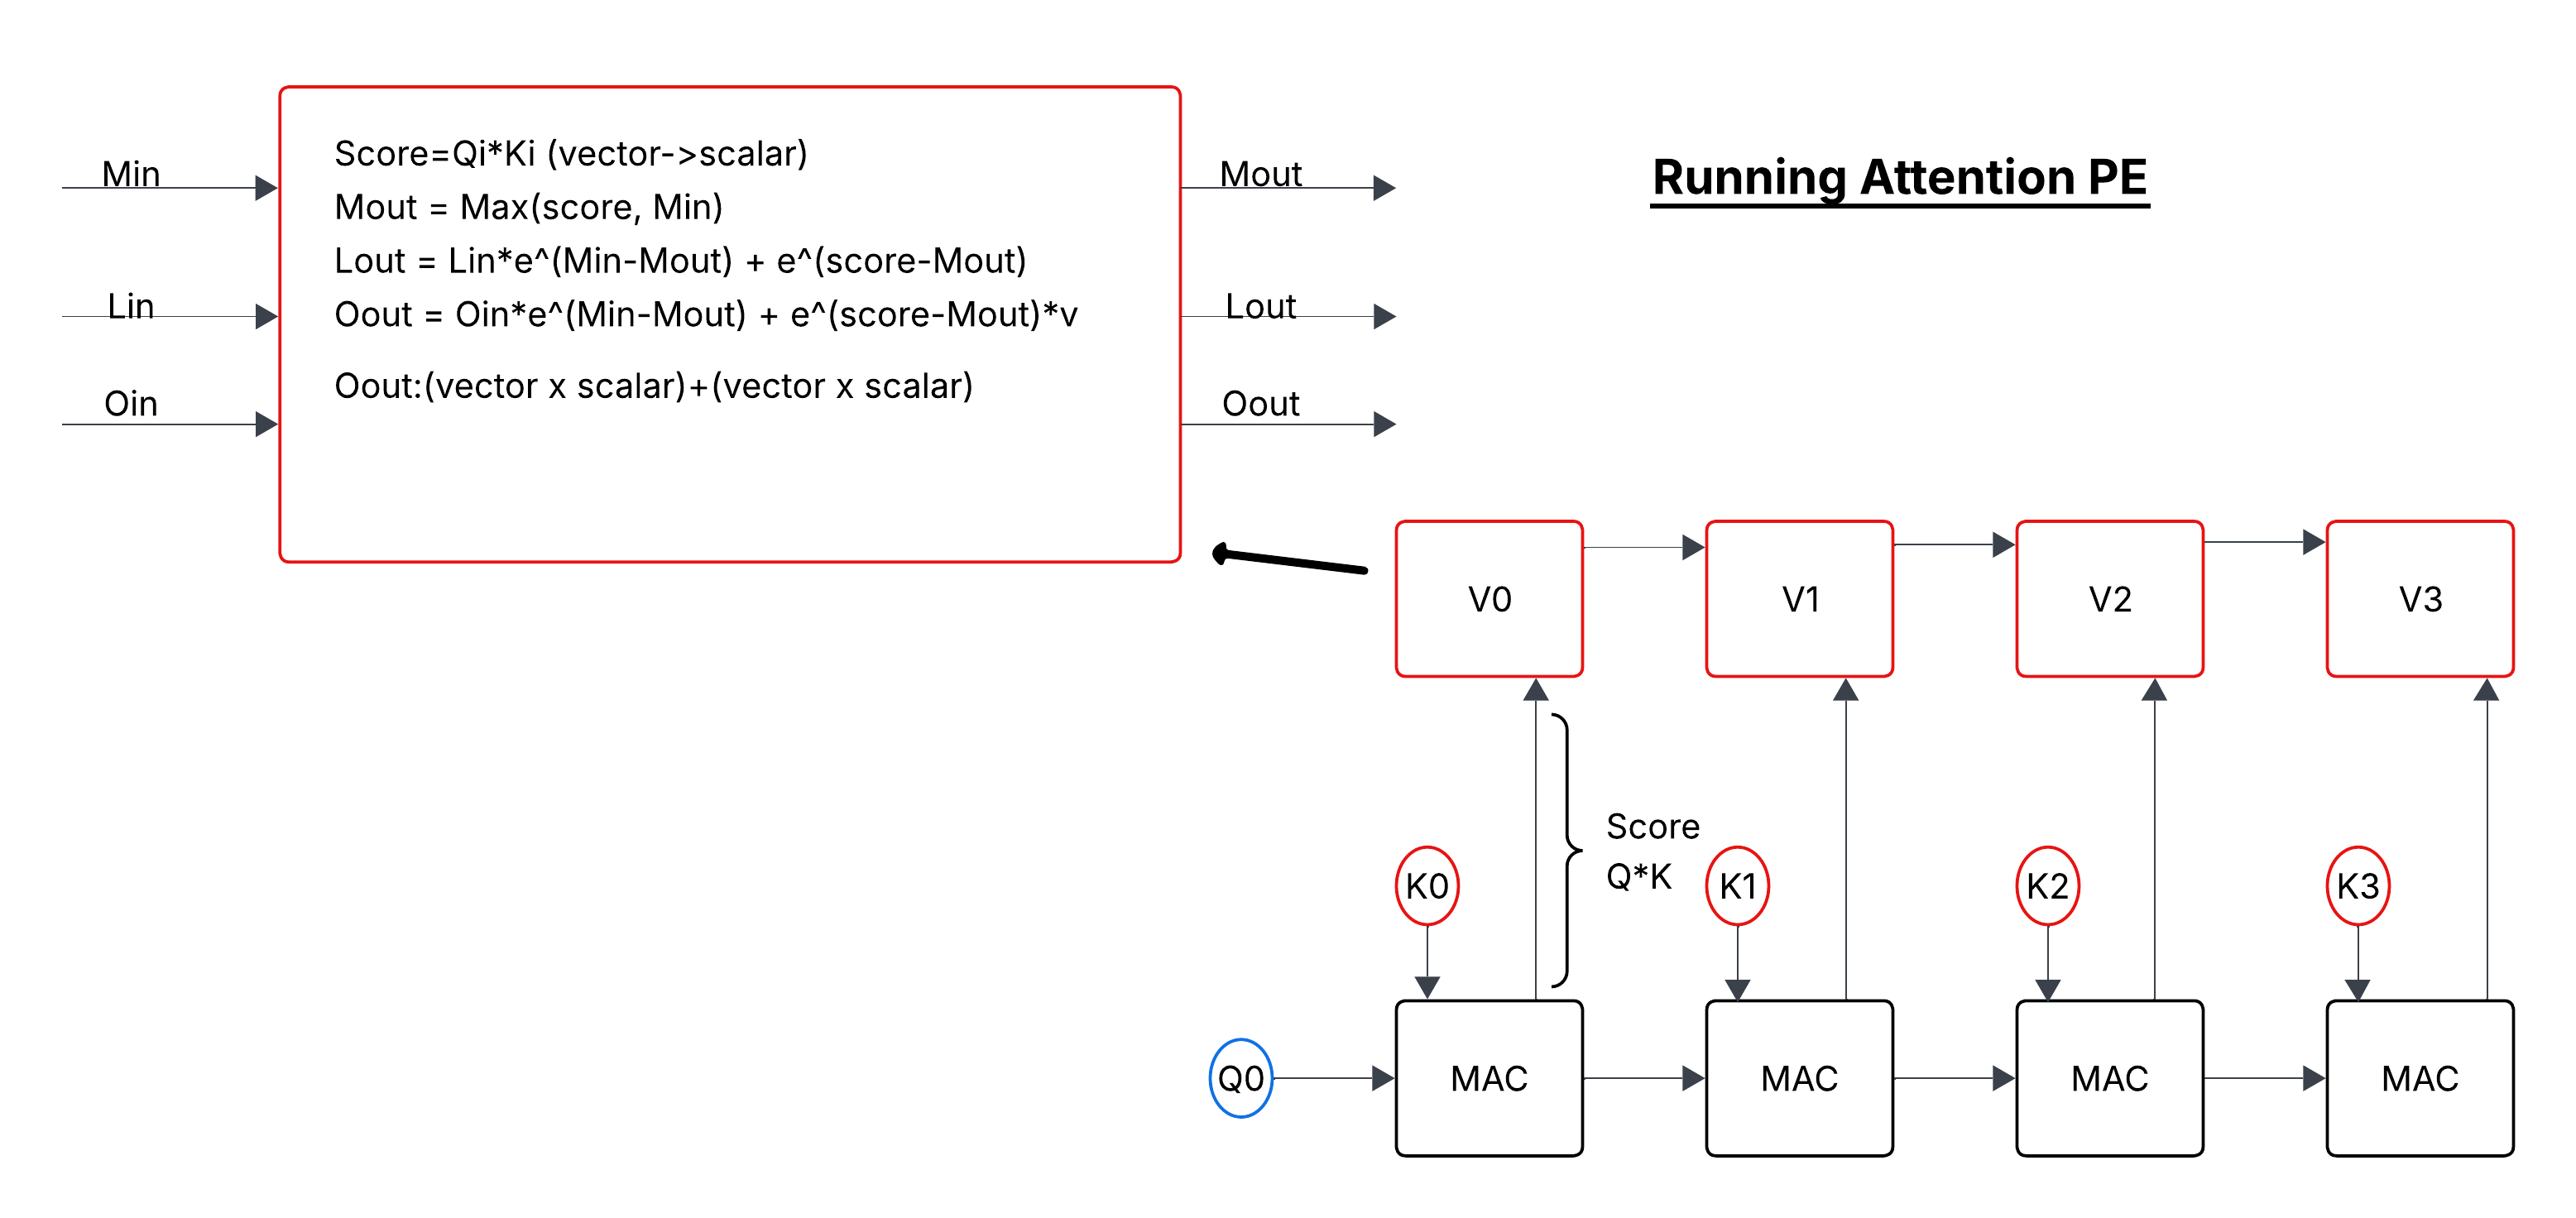
\includegraphics[width=\textwidth]{AttentionPE.png}
        \caption{\textbf{Running Attention PE.}
        Query \(Q_0\) (blue) streams left-to-right past stationary
        \(K_i, V_i\) (red). Stage~1 computes \(s_i = Q \cdot K_i\);
        Stage~2 updates the online softmax state \((m, l, O)\)
        and forwards it to the next column.}
        \label{fig:attention_pe}
    \end{subfigure}
    \hfill
    \begin{subfigure}[t]{0.48\textwidth}
        \centering
        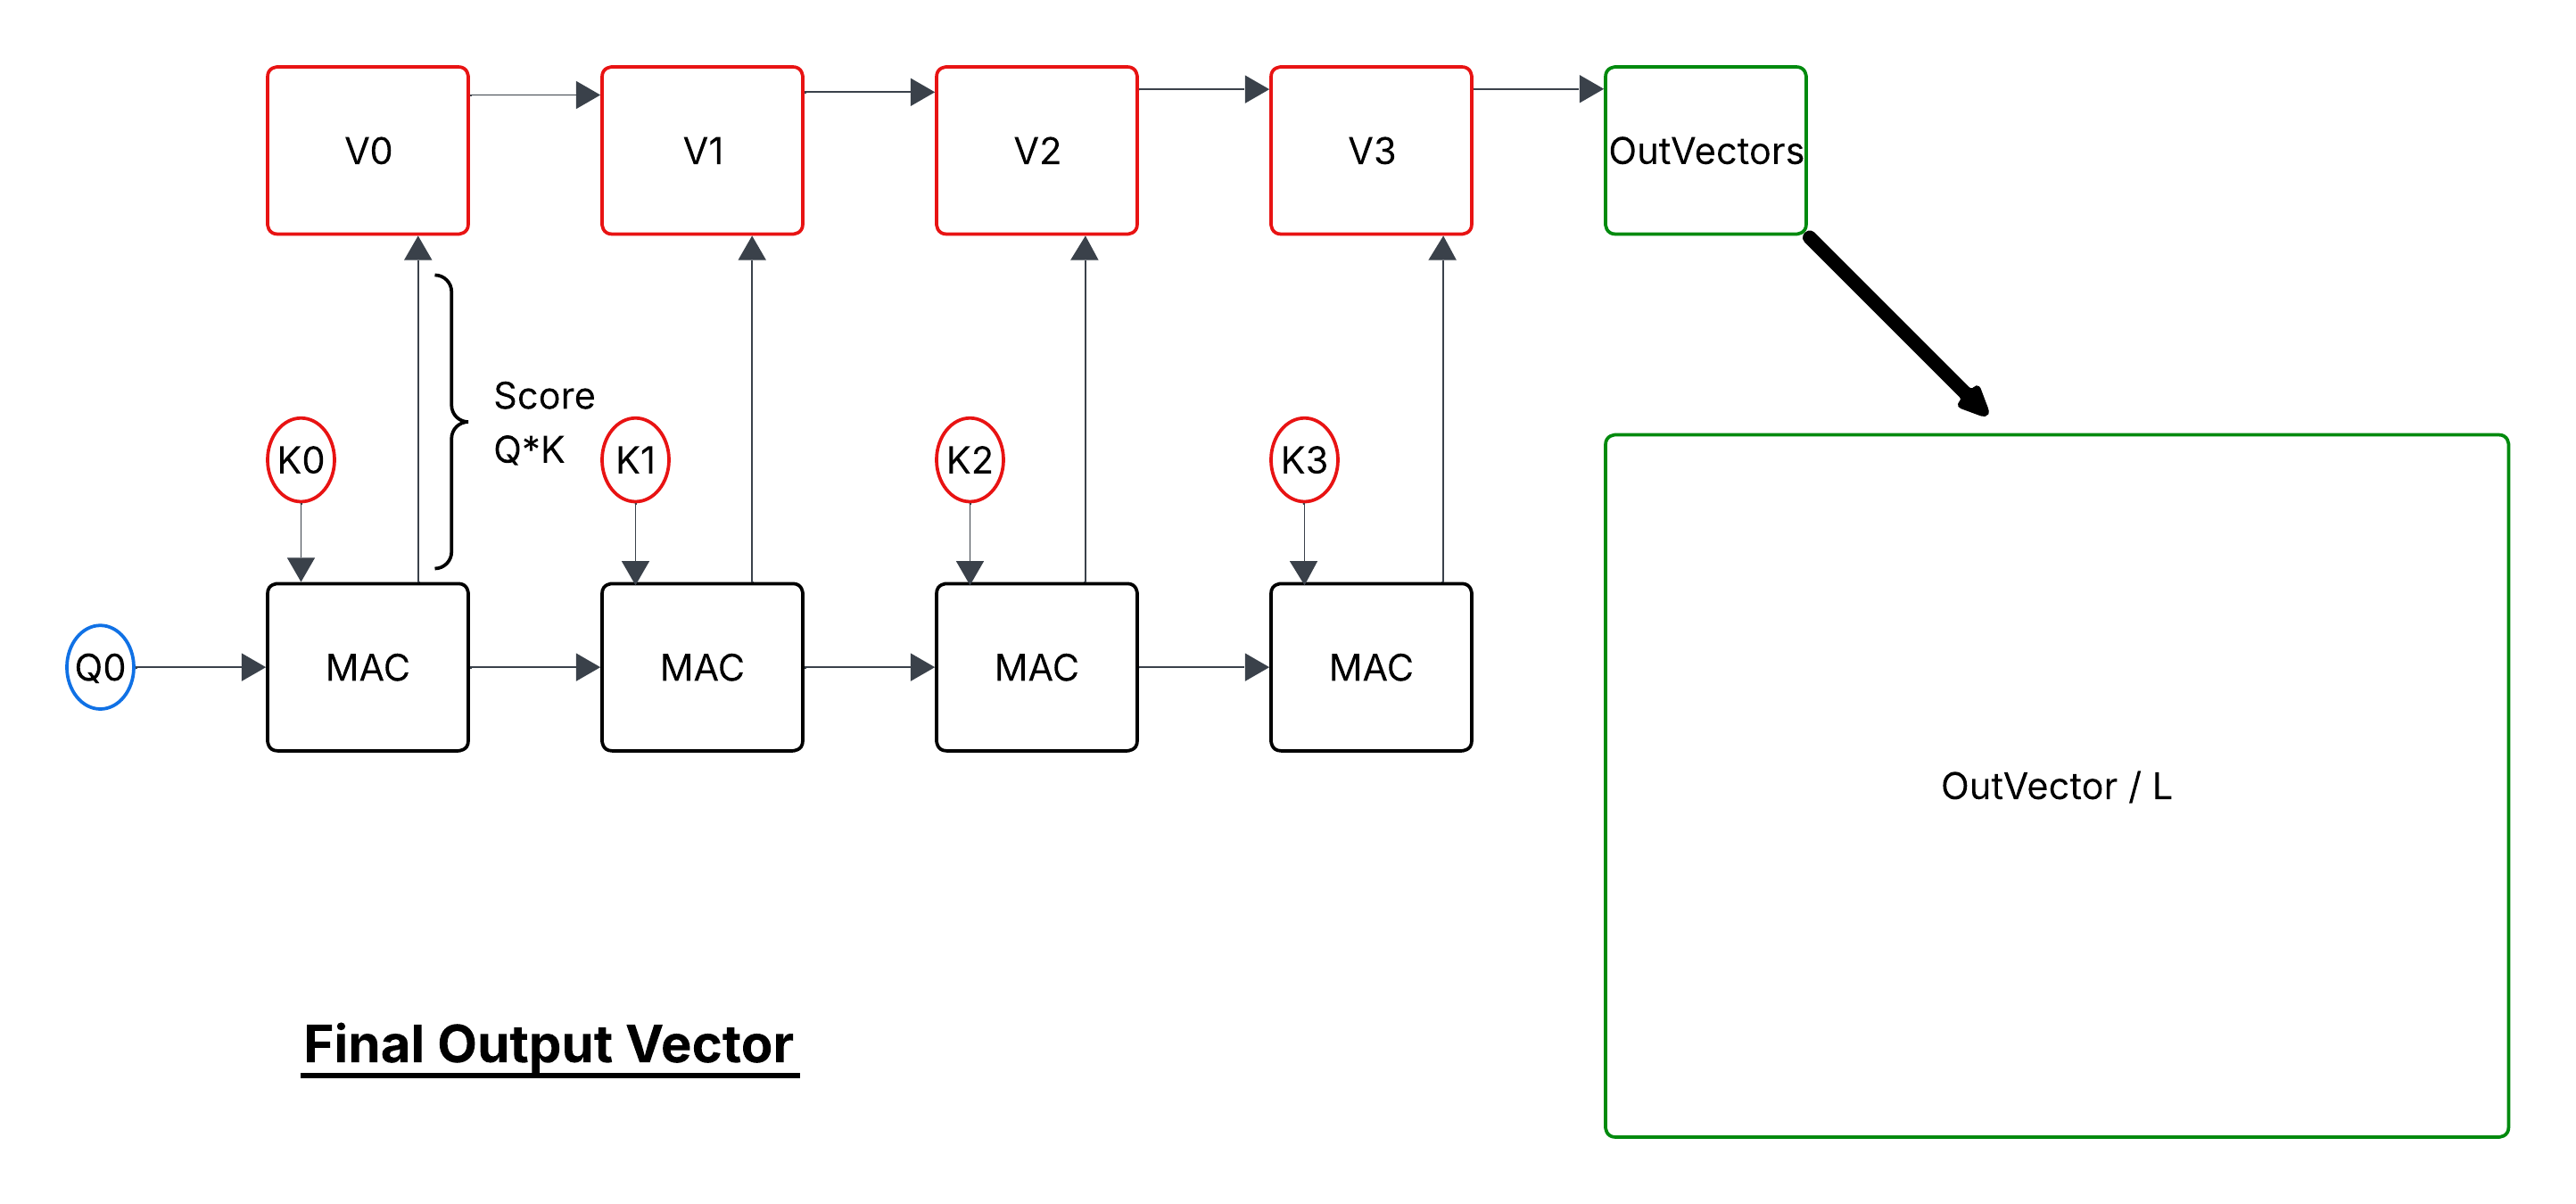
\includegraphics[width=\textwidth]{FinalOutVector.png}
        \caption{\textbf{Final output vector.}
        After traversing all columns the accumulated running state
        is normalised: \(\text{Output} = O_N / l_N\).
        No score matrix is written to DRAM at any point.}
        \label{fig:final_output}
    \end{subfigure}

    \vspace{0.8em}

    % Row 2
    \begin{subfigure}[t]{0.48\textwidth}
        \centering
        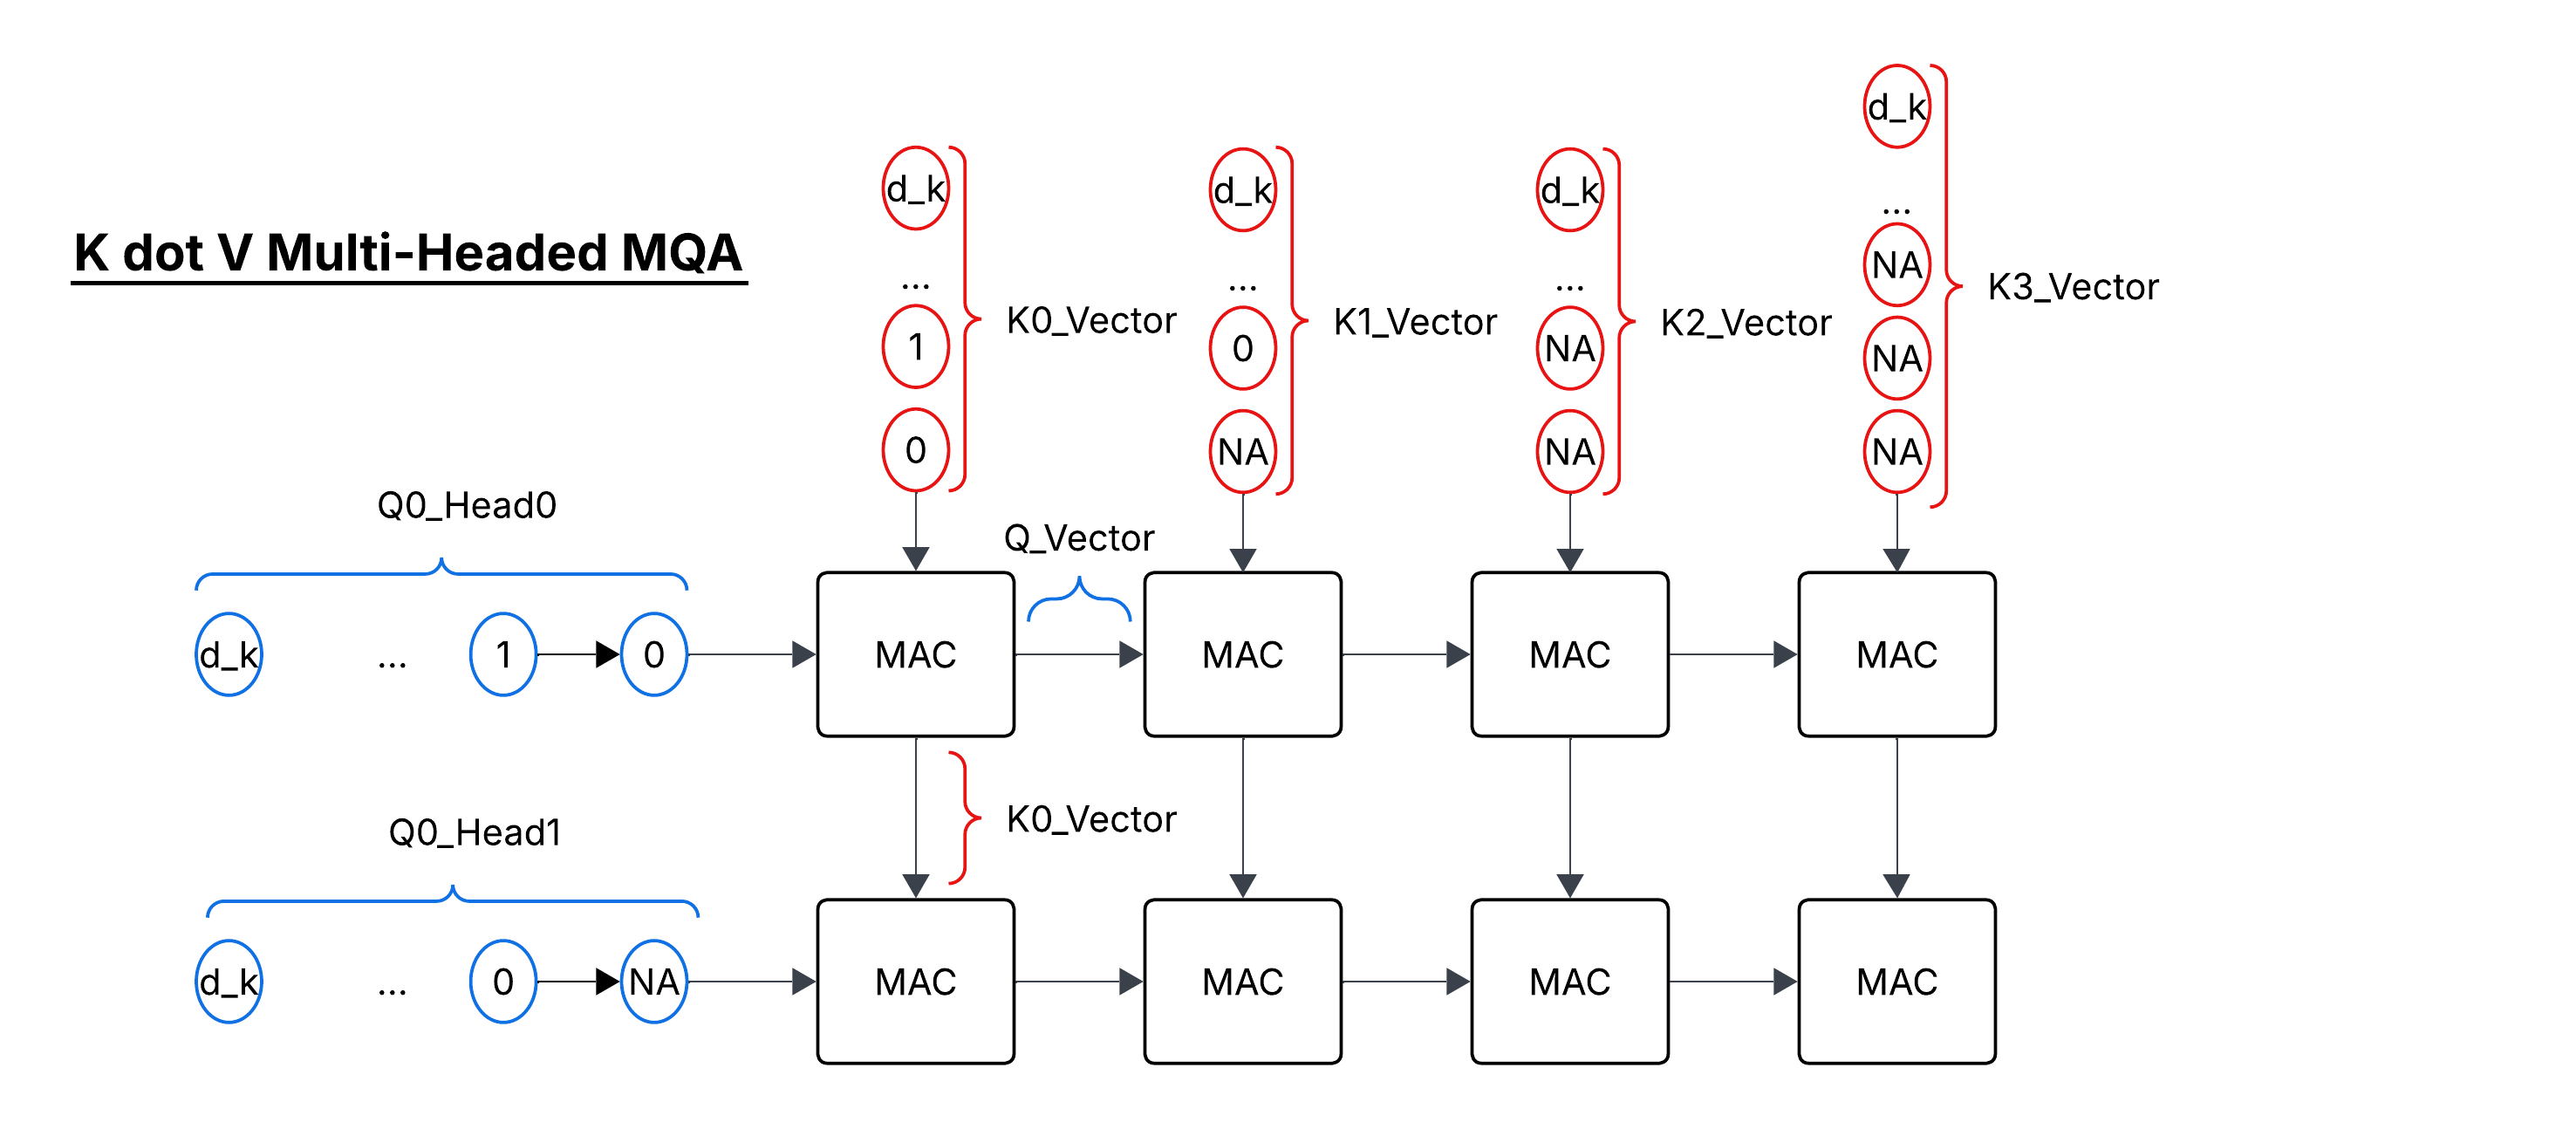
\includegraphics[width=\textwidth]{MultiHeaded.png}
        \caption{\textbf{Multi-headed MQA mapping.}
        Each query head occupies a dedicated row lane.
        All heads share the same stationary \(K_i, V_i\) columns
        (MQA property), so KV is loaded once regardless of head count.}
        \label{fig:multiheaded}
    \end{subfigure}
    \hfill
    \begin{subfigure}[t]{0.48\textwidth}
        \centering
        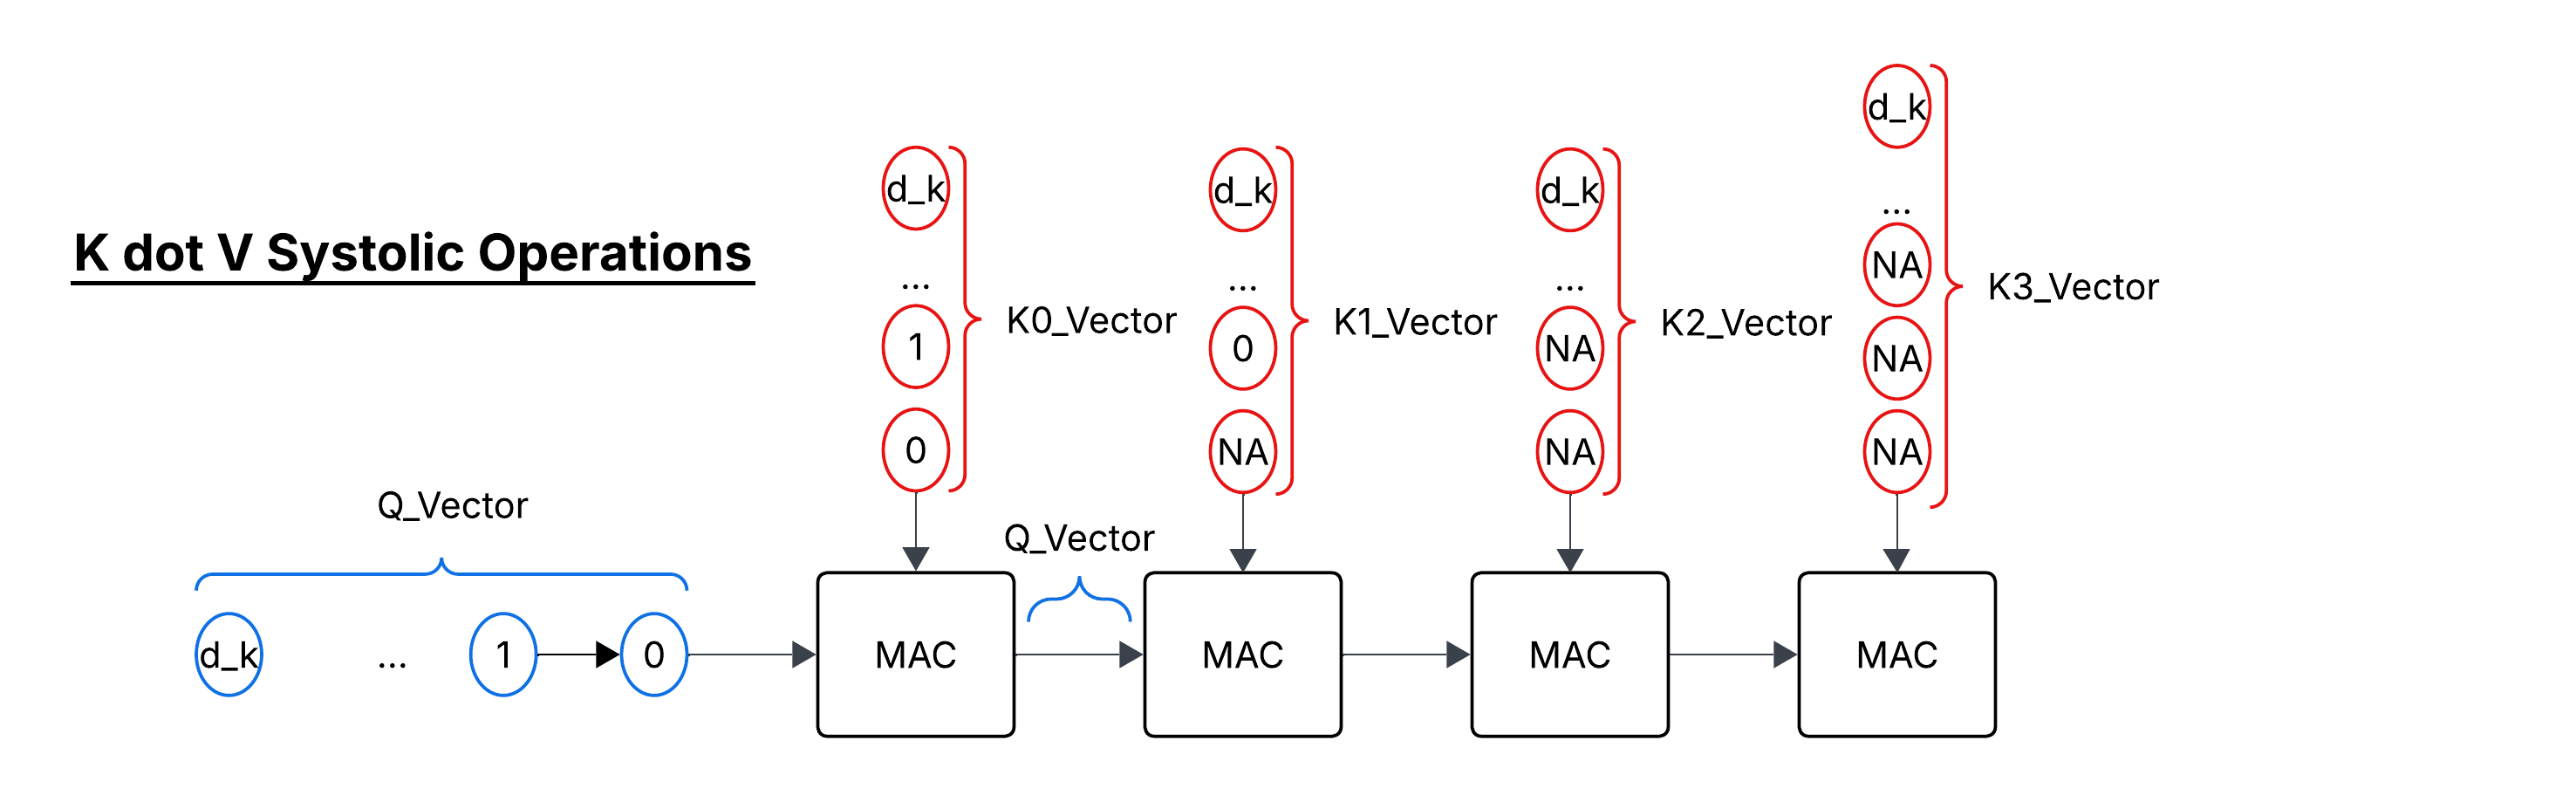
\includegraphics[width=\textwidth]{SystolicSingle.png}
        \caption{\textbf{Single-head systolic operation.}
        The query vector streams through a MAC row, accumulating
        \(Q \cdot K\) element-by-element. The completed score
        propagates upward to its Running Attention PE column.}
        \label{fig:systolic_single}
    \end{subfigure}

    \caption{KV-stationary MQA dataflow. Keys and values remain
    stationary in array columns; query vectors stream left-to-right.
    Online softmax is computed inline at every column, eliminating
    the \(H \times T^2\) score-matrix DRAM traffic of an unfused baseline.}
    \label{fig:kv_stationary_architecture}
\end{figure}

\begin{figure}[H]
    \centering
    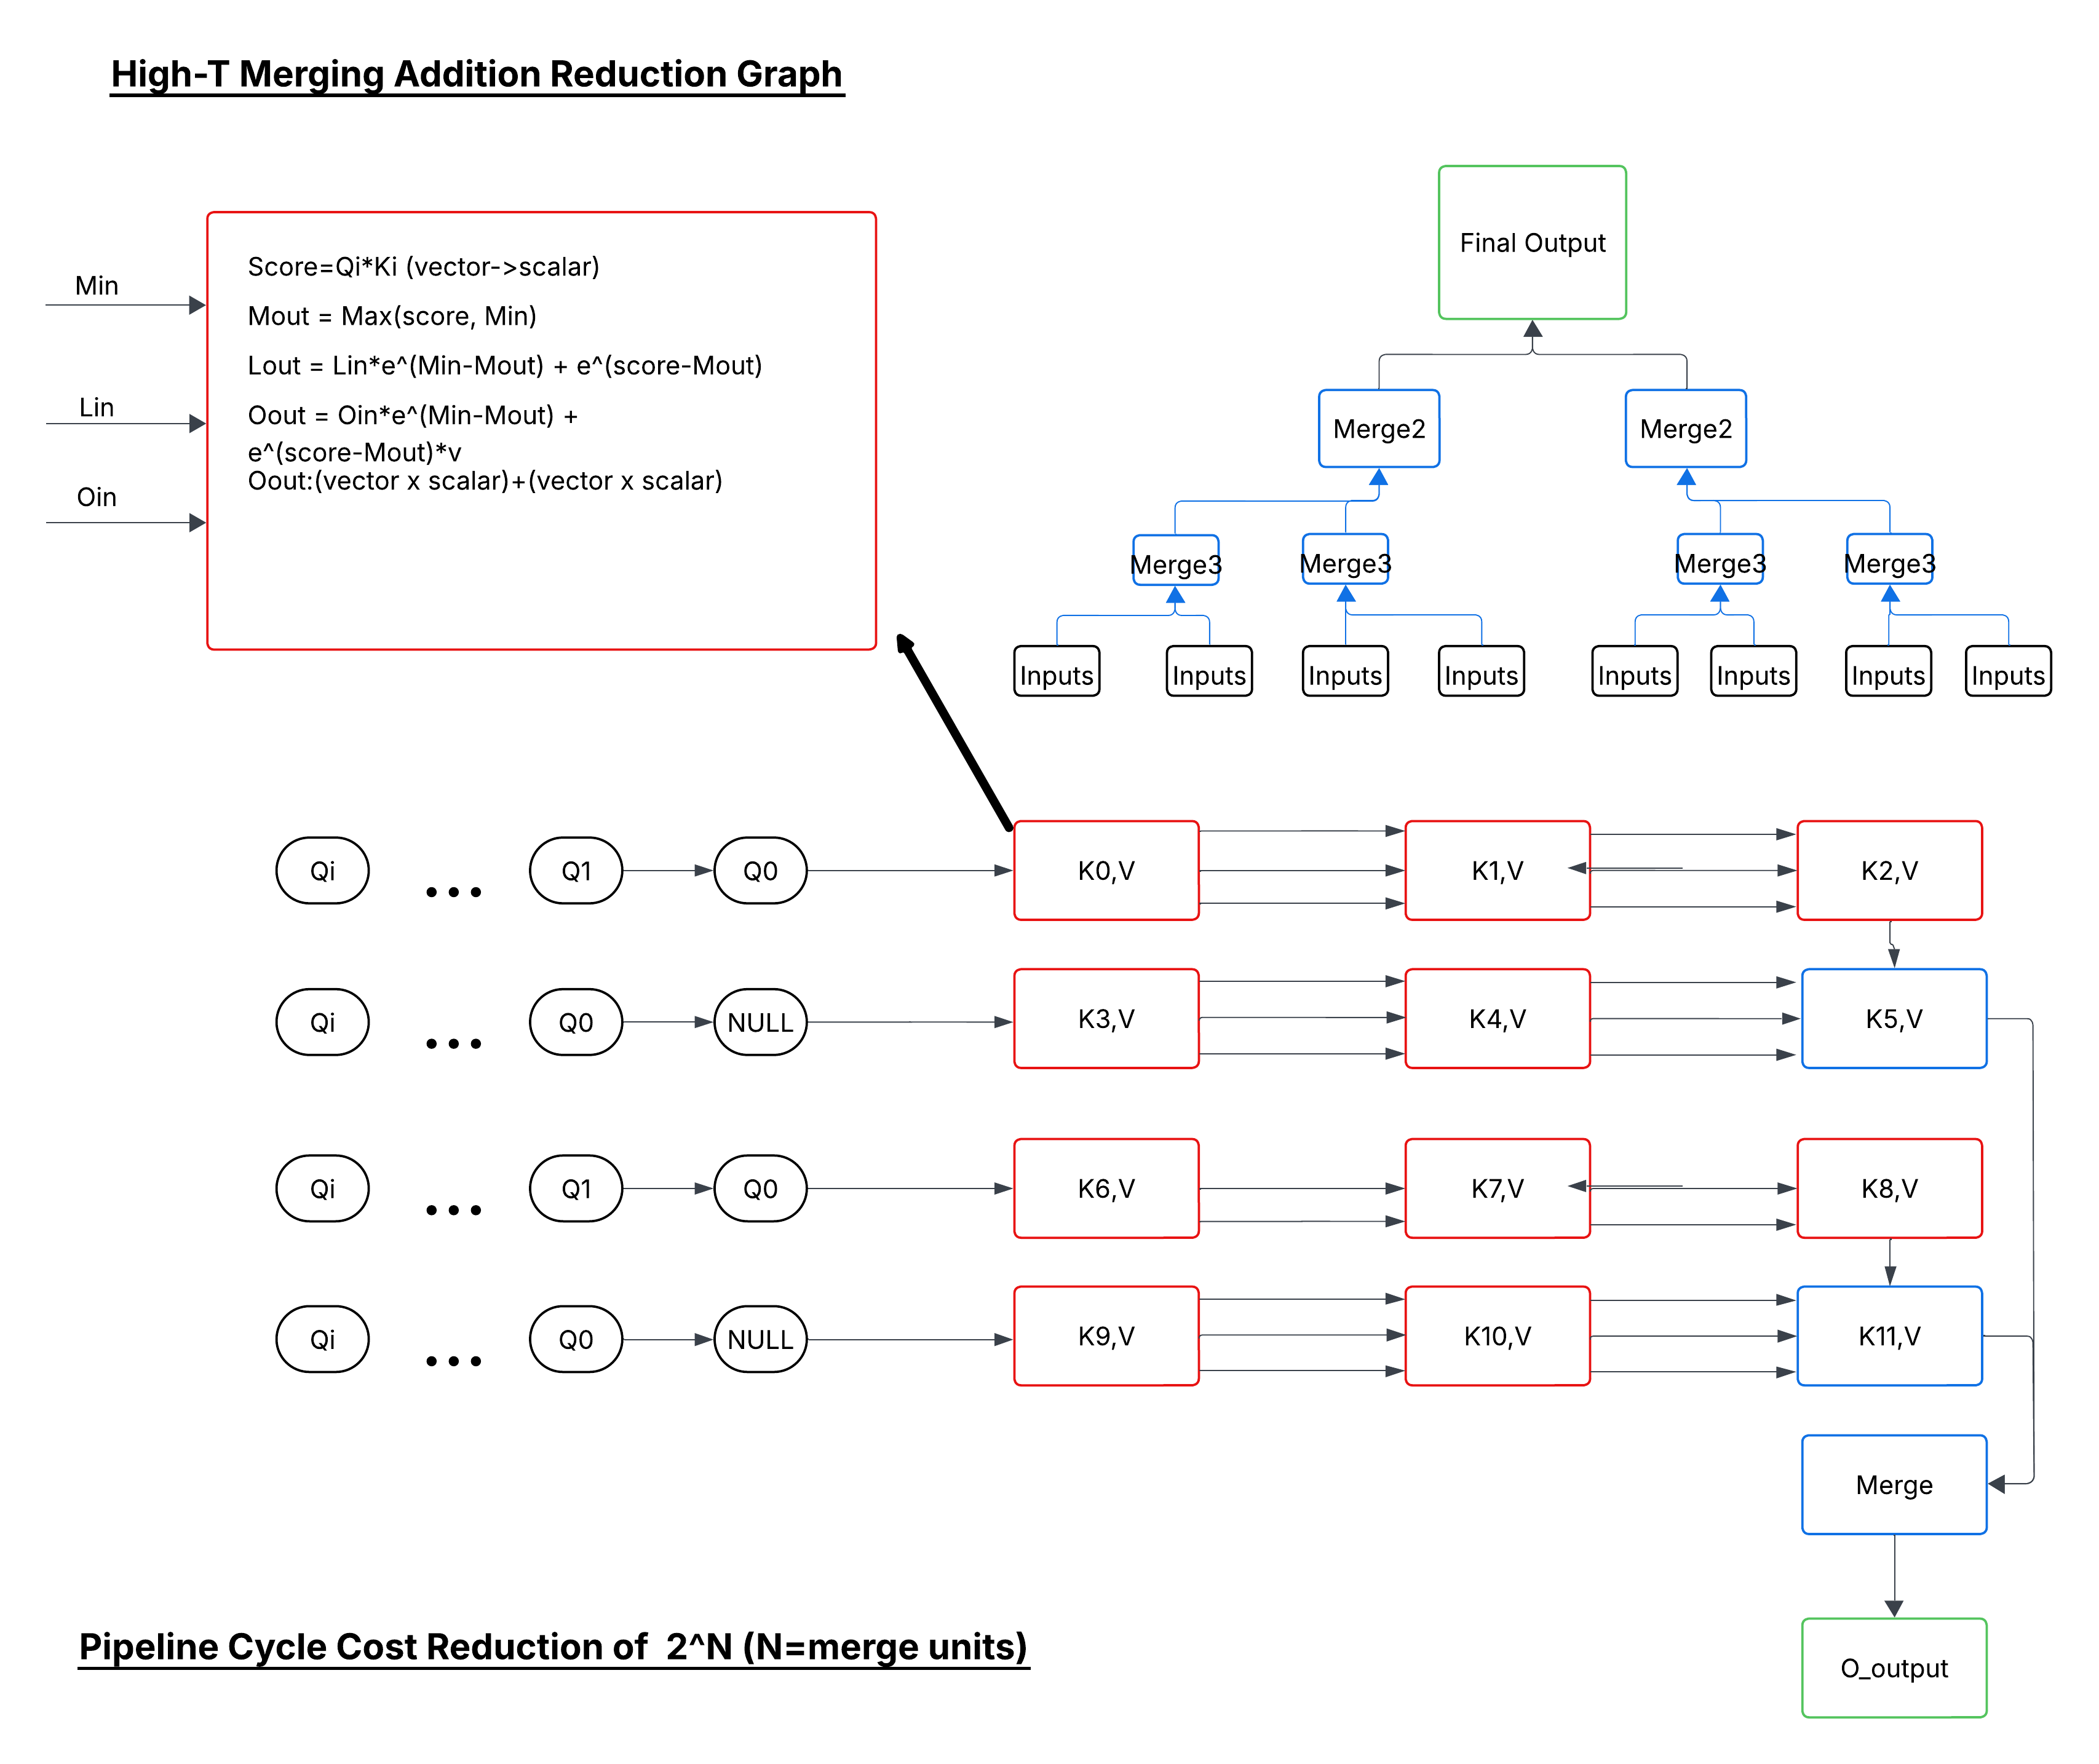
\includegraphics[width=0.82\textwidth]{MergeReductionGraph.png}
    \caption{\textbf{High-\(T\) merge reduction graph} (\(n = 2\) levels shown).
    Four sub-arrays (red KV rows) each process \(T/4\) tokens independently.
    A two-level binary tree of inline merge PEs (blue) combines partial
    \((m, l, O)\) states, cutting per-sub-array drain from \(T-1\) to
    \(T/2^n - 1\) steps at the cost of \(2^n\times\) more PE rows.}
    \label{fig:merge_reduction}
\end{figure}

% ============================================================
\section{Experimental Methodology}
\label{sec:methodology}

\subsection{Hybrid Analytical and SCALE-Sim Model}

The performance model combines an analytical pipeline timing
model with SCALE-Sim cycle-accurate validation for the
compute-dominant GEMM components.

\textbf{SCALE-Sim validated components:}
\begin{itemize}[noitemsep]
    \item Lower MAC unit --- the \(Q \cdot K\) dot-product GEMM,
          mapped as shape \((H \cdot Q_T / lmc) \times d \times \text{eff\_cols}\)
          on a weight-stationary \(H \times \text{eff\_cols}\) array.
    \item FlashAttention QK tile and AV tile --- both mapped as
          independent GEMMs on a \(64 \times 64\) reference array.
\end{itemize}

\textbf{Analytical components:}
\begin{itemize}[noitemsep]
    \item Upper PE latency: \(\tau_{\exp} + \lceil 3d / w \rceil = 7\) cycles.
    \item Full pipeline timing: fill, steady-state, and flush phases
          computed from the two-rate model (\S3.2).
    \item Merge-tree synchronization overhead.
\end{itemize}

The corrected pipeline total substitutes the SCALE-Sim lower-MAC
measurement for the analytical estimate:

\[
\text{corrected\_cycles}
= \text{pipeline\_cycles} - \text{analytical\_mac} + \text{ss\_mac\_cycles}
\]

\subsection{Validation Error Analysis}

The analytical lower-MAC bound is:

\[
\text{analytical\_mac} = \left\lceil Q_T \cdot d \;/\; lmc \right\rceil
\]

This counts pure computation cycles and excludes pipeline drain ---
the time the last packet takes to flush through the remaining
\(\text{eff\_cols} - 1\) columns after the array stops accepting
new work.
SCALE-Sim includes this drain, so its cycle count is always
\(\geq\) the analytical prediction.
The percentage error is:

\[
\delta\% = 100 \cdot
\frac{\text{ss\_mac\_cycles} - \text{analytical\_mac}}
     {\text{analytical\_mac}}
\]

As sequence length grows, the computation term dominates and
drain becomes a smaller fraction of total cycles;
error converges toward zero at large \(T\).
Observed errors for the prefill configurations:
\(lmc = 1\): \(<3\%\) at \(T \geq 512\);
\(lmc = 16\): \(4\)--\(9\%\) at \(T \geq 1{,}024\).

Decode configurations show errors of hundreds to thousands
of percent because the analytical lower-MAC formula counts only
\(d = 128\) MAC cycles while SCALE-Sim measures the full
\(\text{eff\_cols}\)-column pipeline traversal.
Decode behavior is therefore \textbf{not validated} in this work.
Validating the full decode pipeline --- including the interaction
between on-chip KV retention, SRAM capacity constraints, and
multi-pass scheduling --- is left as future work (\S\ref{sec:future}).

\subsection{Fixed Hardware Parameters}

All experiments use the following hardware constants,
chosen to model a realistic edge-inference accelerator:

\begin{center}
\begin{tabular}{ll}
\toprule
Parameter & Value \\
\midrule
Query heads \(H\) & 64 \\
Head dimension \(d\) & 128 \\
Precision & FP16 (2 bytes/element) \\
DRAM bandwidth & 512 B/cycle \\
Upper PE MAC width \(w\) & 128 (fully parallel) \\
Exp lookup latency \(\tau_{\exp}\) & 4 cycles \\
\bottomrule
\end{tabular}
\end{center}

\subsection{Parameter Sweep}

A total of 29 configurations were swept, covering all
combinations of:

\begin{center}
\begin{tabular}{ll}
\toprule
Parameter & Values \\
\midrule
Sequence length \(T\) & 128, 512, 1024, 2048, 4096, 8192 \\
Merge extensions \(n\) & 0 (flat array), 3 (binary tree) \\
MACs per PE column (\(lmc\)) & 1, 16 \\
Mode & Prefill (\(Q_T = T\)), Decode (\(Q_T = 1\)) \\
\bottomrule
\end{tabular}
\end{center}

SCALE-Sim validation was run where memory constraints
permitted (operand matrices below 500\,MB).
Configurations exceeding this limit are reported from the
analytical model only and are flagged accordingly.

\subsection{Experiments Conducted}

Three distinct experiments were run, each targeting a different
layer of the model.

\textbf{Experiment 1 --- Lower MAC validation (29 configurations).}
Each configuration maps the Q·K dot-product GEMM onto SCALE-Sim
as a weight-stationary array of shape \(H \times \text{eff\_cols}\)
with GEMM dimensions \(M = H \cdot Q_T / lmc\), \(N = \text{eff\_cols}\),
\(K = d\).
The analytical prediction \(\lceil Q_T \cdot d / lmc \rceil\) is
compared against SCALE-Sim compute cycles;
the delta is recorded as the drain-overhead error~\(\delta\%\).
Of 29 configurations, 16 prefill runs completed successfully;
decode runs were excluded after all 12 showed divergence exceeding
200\% (see \S4.2).
Selected prefill validation results are shown in
Table~\ref{tab:mac_validation}.

\begin{table}[H]
\centering
\caption{Lower MAC SCALE-Sim validation --- selected prefill configurations.
\(\delta\%\) = drain overhead as a percentage of the analytical MAC bound.
Mac frac = SCALE-Sim MAC cycles as a fraction of corrected total pipeline cycles.}
\label{tab:mac_validation}
\begin{tabular}{rrrrrrr}
\toprule
\(T\) & \(n\) & \(lmc\) & Analytical & SCALE-Sim & \(\delta\%\) & Mac frac \\
\midrule
128  & 0 &  1 & 16,384 & 16,891 & 3.1\%  & 40.2\% \\
128  & 0 & 16 &  1,024 &  1,531 & 49.5\% &  5.7\% \\
512  & 0 &  1 & 65,536 & 66,811 & 1.9\%  & 46.7\% \\
512  & 0 & 16 &  4,096 &  5,371 & 31.1\% &  6.6\% \\
1024 & 0 & 16 &  8,192 & 10,491 & 28.1\% &  6.8\% \\
2048 & 0 & 16 & 16,384 & 20,731 & 26.5\% &  6.9\% \\
2048 & 3 & 16 & 16,384 & 17,147 &  4.7\% &  3.6\% \\
4096 & 3 & 16 & 32,768 & 34,043 &  3.9\% &  3.9\% \\
8192 & 3 & 16 & 65,536 & 67,835 &  3.5\% &  4.0\% \\
\bottomrule
\end{tabular}
\end{table}

Two patterns are visible.
First, \(lmc = 1\) error converges quickly: \(<3\%\) at \(T \geq 512\)
because the MAC computation dominates and drain is a small fraction.
Second, \(lmc = 16\) shows higher error at small \(T\) (49\% at
\(T=128\)) but converges by \(T = 1{,}024\) (\(<7\%\)) as the
computation term grows relative to the fixed drain overhead.
The Mac frac column shows the lower MAC unit accounts for only
4--7\% of total pipeline cycles in the corrected model for
\(lmc = 16\) --- the bottleneck is the upper PE and pipeline
fill/drain, not the dot product.

\textbf{Experiment 2 --- Prefill vs FlashAttention sweep (24 configurations).}
KV-stat is compared against a FlashAttention-style fused reference
across all \((T, n, lmc)\) combinations.
Both architectures use a \(64 \times 64\) FlashAttention tile
(SRAM-constrained to \(H = 64\) tile size).
The KV-stat corrected cycle count from Experiment~1 is used where
SCALE-Sim was available; the analytical pipeline total is used
otherwise.
Results are reported as raw speedup, PE area ratio, and
area-normalized speedup (Table~\ref{tab:prefill_results}).
Of 24 configurations, 15 use SCALE-Sim-corrected KV-stat cycles;
9 use analytical estimates only (flagged in the table).

\textbf{Experiment 3 --- Cycle breakdown decomposition.}
For each validated configuration the total pipeline cycles are
decomposed into three additive terms:
(i) SCALE-Sim lower MAC cycles (\texttt{ss\_lower\_mac}),
(ii) within-row stagger cost \((P-1) \cdot \text{packet\_stagger}\),
and (iii) upper PE and pipeline fill/drain overhead.
This decomposition confirms that for \(n=3, lmc=16\) the lower MAC
and stagger costs are roughly equal --- the pipeline is balanced
--- while for \(n=0, lmc=16\) at large \(T\), stagger cost
dominates, identifying the upper PE as the throughput bottleneck.

% ============================================================
% PE UTILIZATION FIGURE
% ============================================================

\begin{figure}[H]
    \centering
    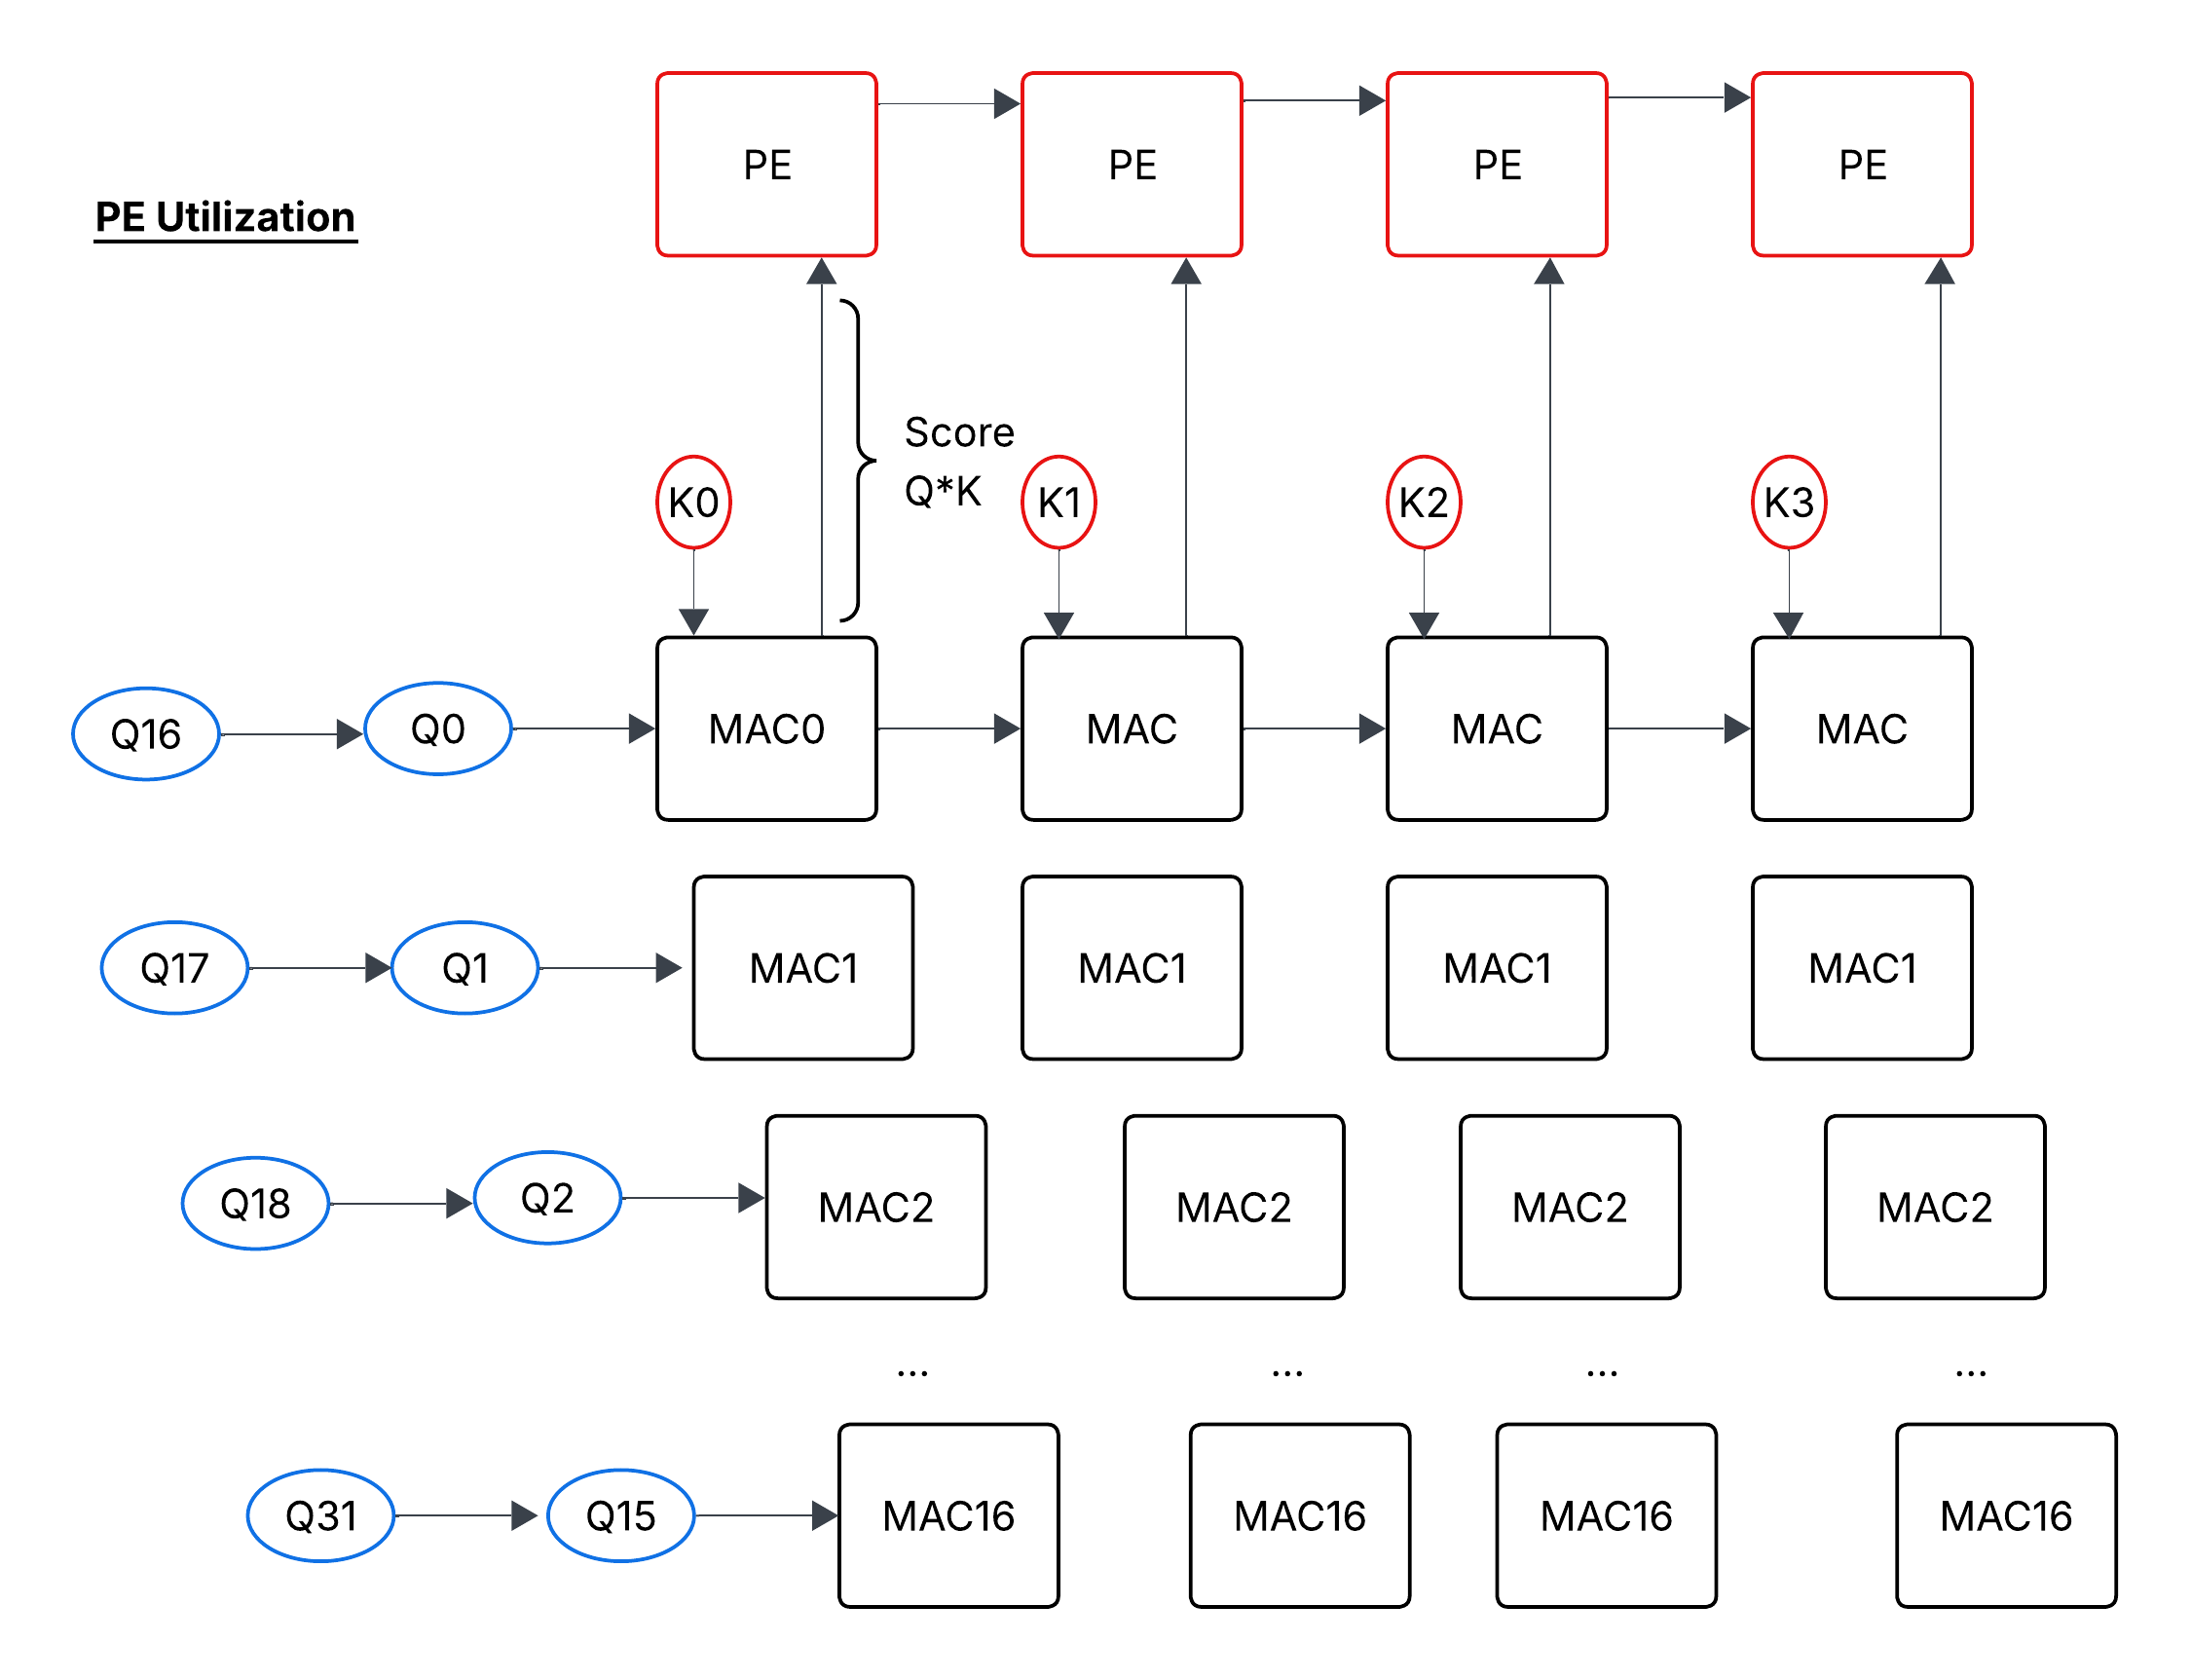
\includegraphics[width=0.82\textwidth]{PEUtilization.png}
    \caption{\textbf{PE utilization with \(lmc = 16\) interleaved MAC rows.}
    Sixteen query packets (\(Q_0\)--\(Q_{15}\)) are time-multiplexed through
    the same column, each staggered by \(\lceil d/16 \rceil = 8\) cycles.
    Initiation interval drops from 128 to 8 cycles; upper Running Attention
    PE utilisation rises from \(\approx\)5\% to \(\approx\)87.5\%.
    All rows share a single on-chip K register --- no K duplication required.}
    \label{fig:pe_utilization}
\end{figure}

% ============================================================
\section{Results}
\label{sec:results}

\subsection{Baseline Characterization}
\label{subsec:baseline}

Three baseline variants are used throughout the comparison,
each representing a distinct hardware or software assumption.

\textbf{Variant~1 --- Original \(64 \times 64\), unfused.}
A 4,096 MAC weight-stationary array running two sequential GEMMs
(Q·K\(^\top\), then scores·V) with the full score matrix written
to and read back from DRAM between them.
This is the default SCALE-Sim reference configuration.

\textbf{Variant~2 --- MAC-normalized, unfused.}
Same two-GEMM structure with the array resized to match
KV-stat's MAC count: \(8{,}192 \times (T/8)\) = 8.4M MACs
at \(T = 8{,}192\).
This isolates architectural efficiency from raw compute budget.

\textbf{Variant~3 --- MAC-normalized, fused.}
Same large array as Variant~2 with FlashAttention-style tiling:
no score matrix written to DRAM.
This is the fairest possible comparison --- equal MACs,
equal memory discipline.

\subsubsection*{The \(64 \times 64\) Baseline Is Compute-Bound at Every \(T\)}

The original \(64 \times 64\) array is perpetually compute-bound:
its 4,096 MACs cannot keep pace with the prefill workload at any
tested sequence length.

\begin{table}[H]
\centering
\caption{Original \(64 \times 64\) unfused baseline roofline analysis
across all sequence lengths (prefill, \(H=64\), \(d=128\), FP16).}
\label{tab:baseline_orig}
\begin{tabular}{rrrrr}
\toprule
\(T\) & Compute cycles & Memory cycles & Estimated cycles & Bottleneck \\
\midrule
128   &      65,536 &      16,512 &      65,536 & COMPUTE \\
512   &   1,048,576 &     164,352 &   1,048,576 & COMPUTE \\
1,024 &   4,194,304 &     590,848 &   4,194,304 & COMPUTE \\
2,048 &  16,777,216 &   2,230,272 &  16,777,216 & COMPUTE \\
4,096 &  67,108,864 &   8,654,848 &  67,108,864 & COMPUTE \\
8,192 & 268,435,456 &  34,086,912 & 268,435,456 & COMPUTE \\
\bottomrule
\end{tabular}
\end{table}

At \(T = 8{,}192\) the compute bottleneck is \(7.8\times\) worse
than the memory bottleneck.
Comparing KV-stat (memory-bound, 8.4M MACs) against this baseline
guarantees a large speedup regardless of architectural quality;
the 511$\times$ speedup figure is almost entirely a MAC-count artifact.

\subsubsection*{Score-Matrix Dominance}

Once MACs are equalized, the unfused baseline immediately flips
to memory-bound --- and the score matrix accounts for essentially
all of the DRAM traffic.
At \(T = 8{,}192\):

\begin{table}[H]
\centering
\caption{DRAM traffic breakdown for the MAC-normalized unfused baseline
at \(T = 8{,}192\), \(H=64\), \(d=128\), FP16.}
\label{tab:dram_breakdown}
\begin{tabular}{lrr}
\toprule
Traffic component & Size (MB) & \% of total \\
\midrule
Score matrix (write + read) & 17,179.9 & 98.4\% \\
Q reads                     &    134.2 &  0.77\% \\
Output writes               &    134.2 &  0.77\% \\
K reads                     &      2.1 &  0.01\% \\
V reads                     &      2.1 &  0.01\% \\
\midrule
\textbf{Total}              & \textbf{17,452.5} & \\
\bottomrule
\end{tabular}
\end{table}

The score matrix scales as
\(H \times T^2 \times \text{bpe} \times 2 = 64 \times 8192^2 \times 2 \times 2\)
bytes.
This is why the unfused MAC-normalized baseline is \(65\times\)
slower than KV-stat: 17.45\,GB vs 0.27\,GB at the same bandwidth.

\subsubsection*{Fused Baseline Closes the Gap}

The fused (FlashAttention-style) baseline eliminates score-matrix
traffic entirely, dropping total DRAM to 272.6\,MB --- identical
to KV-stat.
Arithmetic intensity jumps from 63 to 4,033 MACs/byte.
Table~\ref{tab:ai_comparison} compares all four architectures
at \(T = 8{,}192\).

\begin{table}[H]
\centering
\caption{Arithmetic intensity at \(T = 8{,}192\), \(H=64\), \(d=128\), FP16.
KV-stat has \(2\times\) the MACs of the baselines (dot product + value accumulation)
but the same 0.27\,GB DRAM as the fused baseline, giving \(2\times\) higher AI.}
\label{tab:ai_comparison}
\begin{tabular}{lrrr}
\toprule
Configuration & Total MACs & Total DRAM & AI (MACs/byte) \\
\midrule
\(64 \times 64\) unfused    & 1.10T & 17.45\,GB & 63 \\
MAC-norm unfused            & 1.10T & 17.45\,GB & 63 \\
MAC-norm fused              & 1.10T &  0.27\,GB & 4,033 \\
KV-stat \(n=3,\;lmc=16\)   & 2.20T &  0.27\,GB & 8,066 \\
\bottomrule
\end{tabular}
\end{table}

\subsubsection*{Three-Way Speedup Summary}

Table~\ref{tab:speedup_3way} shows the speedup of KV-stat
(\(n=3, lmc=16\), pipeline cycles) against all three baseline
variants.
The three columns tell three different stories:
the first is misleading, the second is real but driven by
score-matrix traffic, and the third is the honest comparison
after equal fusion.

\begin{table}[H]
\centering
\caption{Three-way prefill speedup: KV-stat \(n=3,\;lmc=16\)
pipeline cycles vs each baseline variant.
Below \(T=2{,}048\) KV-stat is slower than the fused baseline;
the pipeline fill overhead is not yet amortized.}
\label{tab:speedup_3way}
\begin{tabular}{rrrr}
\toprule
\(T\) & vs \(64{\times}64\) unfused & vs MAC-norm unfused & vs MAC-norm fused \\
\midrule
128   &  0.9$\times$ &  0.2$\times$ & 0.12$\times$ \\
512   & 12.8$\times$ &  2.0$\times$ & 0.41$\times$ \\
1,024 & 44.4$\times$ &  6.3$\times$ & 0.70$\times$ \\
2,048 & 127.8$\times$ & 17.0$\times$ & \textbf{1.01$\times$} \\
4,096 & 255.5$\times$ & 33.0$\times$ & \textbf{1.01$\times$} \\
8,192 & 511.0$\times$ & 64.9$\times$ & \textbf{1.01$\times$} \\
\bottomrule
\end{tabular}
\end{table}

The fused-baseline crossover at \(T = 2{,}048\) is the true
breakeven for the KV-stat \(n=3\) configuration.
For the flatter \(n=0, lmc=16\) design the crossover occurs
earlier (between \(T=1{,}024\) and \(T=2{,}048\)) owing to
its lower pipeline fill overhead.

\subsection{Prefill: KV-Stationary vs FlashAttention on Equal Silicon}

The primary comparison pairs KV-stat against a FlashAttention-style
fused baseline.
Both architectures eliminate score-matrix DRAM traffic and have
identical DRAM footprints; the comparison is therefore purely on
cycles and PE area.
The FlashAttention reference uses a fixed \(64 \times 64\) array
(4{,}096 PEs); KV-stat scales with \(T\) as described in \S3.

The key metric is \textit{area-normalized speedup}:
raw cycle speedup divided by the PE area ratio.
A value above 1.0 means KV-stat delivers more throughput
per unit silicon than FlashAttention.

\begin{table}[H]
\centering
\caption{Prefill results --- KV-stat vs FlashAttention.
Columns show the raw cycle speedup, PE area multiple,
area-normalized speedup, and SCALE-Sim validation status.
All DRAM footprints are equal (both fused).}
\label{tab:prefill_results}
\begin{tabular}{lrrrrr}
\toprule
Configuration & \(T\) & Raw speedup & PE ratio & Area-norm. & Validated \\
\midrule
\(n=0,\;lmc=1\)  &  512 &  7.6$\times$ &  8$\times$ & 0.95$\times$ & \checkmark \\
\(n=0,\;lmc=16\) &  512 & 13.2$\times$ &  8$\times$ & \textbf{1.65$\times$} & \checkmark \\
\(n=3,\;lmc=16\) &  512 &  6.4$\times$ &  8$\times$ & 0.81$\times$ & \checkmark \\
\midrule
\(n=0,\;lmc=16\) & 1024 & 27.9$\times$ & 16$\times$ & \textbf{1.74$\times$} & \checkmark \\
\(n=3,\;lmc=16\) & 1024 & 16.1$\times$ & 16$\times$ & 1.01$\times$ & \checkmark \\
\midrule
\(n=0,\;lmc=16\) & 2048 & 57.4$\times$ & 32$\times$ & \textbf{1.79$\times$} & \checkmark \\
\(n=3,\;lmc=16\) & 2048 & 36.9$\times$ & 32$\times$ & 1.15$\times$ & \checkmark \\
\midrule
\(n=3,\;lmc=16\) & 4096 & 79.4$\times$ & 64$\times$ & 1.24$\times$ & \checkmark \\
\(n=3,\;lmc=16\) & 8192 & 165.2$\times$ & 128$\times$ & 1.29$\times$ & \checkmark \\
\midrule
\(n=0,\;lmc=16\) & 4096 & 118.2$\times$ & 64$\times$ & \textbf{1.85$\times$} & analytical \\
\(n=0,\;lmc=16\) & 8192 & 238.0$\times$ & 128$\times$ & \textbf{1.86$\times$} & analytical \\
\bottomrule
\end{tabular}
\end{table}

Three findings stand out from Table~\ref{tab:prefill_results}.

\textbf{(1) \(lmc = 16\) is the critical parameter.}
Moving from \(lmc = 1\) to \(lmc = 16\) at \(T = 512\) improves
area-normalized speedup from 0.95$\times$ to 1.65$\times$ ---
a configuration that would otherwise not beat FlashAttention per
unit area.
The gain comes entirely from reducing the column initiation
interval from 128 to 8 cycles, raising upper PE utilization
from 5\% to 87.5\%.

\textbf{(2) Merge extensions hurt area efficiency.}
At \(T = 2{,}048\): \(n = 0, lmc = 16\) achieves 1.79$\times$
area-normalized speedup; \(n = 3, lmc = 16\) achieves only
1.15$\times$.
Merge extensions multiply PE count by \(2^n = 8\times\) while
delivering only a 1.6$\times$ cycle improvement over \(n = 0\).
The simpler flat design is both cheaper and faster per unit area.

\textbf{(3) The advantage grows with sequence length.}
Area-normalized speedup for \(n = 0, lmc = 16\) increases from
1.65$\times$ at \(T = 512\) to 1.79$\times$ at \(T = 2{,}048\)
and extrapolates to 1.86$\times$ at \(T = 8{,}192\)
(unvalidated analytical estimate).
This is consistent with pipeline efficiency improving as the
computation-to-drain ratio increases.

\subsection{Prefill: Comparison Against Unfused Baseline}

The full baseline characterization is presented in
\S\ref{subsec:baseline}.
In summary: the 65$\times$ cycle speedup against the MAC-normalized
unfused baseline at \(T = 8{,}192\) is entirely explained by the
17.45\,GB score-matrix DRAM that the unfused baseline incurs
(98.4\% of its total traffic) vs the 0.27\,GB footprint of KV-stat.
This advantage collapses to \(\sim\)1$\times$ when the baseline
adopts fused (FlashAttention-style) tiling, confirming that the
gain is not unique to the KV-stationary dataflow --- it is the
same score-matrix elimination that FlashAttention achieves in
software.

\subsection{Autoregressive Decode: Analytical Projection (Unvalidated)}

The analytical model projects a significant DRAM reduction for
autoregressive decode if the KV cache is held in on-chip SRAM
across generated tokens.
\textbf{This projection has not been validated with SCALE-Sim};
it is included to motivate the design direction described in
Section~\ref{sec:future}.

At \(T = 8{,}192\), \(H = 64\), \(d = 128\), FP16, the
per-token DRAM costs under the analytical model are:

\begin{center}
\begin{tabular}{lrl}
\toprule
Component & Per-step DRAM & Notes \\
\midrule
Conventional (KV reloaded) & 6.0\,MB & K + V + Q + scores + output \\
KV-stat model (KV in SRAM) & 32\,KB  & Q + output only \\
\midrule
Projected reduction & \textbf{188$\times$} & analytical only \\
\bottomrule
\end{tabular}
\end{center}

The 188$\times$ figure assumes the full KV cache fits in on-chip
SRAM throughout the generation run.
At \(T = 8{,}192\) this requires 128\,MB of on-chip SRAM ---
a substantial area commitment that motivates the two-pass
extension discussed in Section~\ref{sec:future}.

\subsection{Physical Cost}

The area savings implied by the speedup numbers require
substantial silicon.
For the best prefill configuration (\(n = 0, lmc = 16\)) at
\(T = 8{,}192\):

\begin{center}
\begin{tabular}{ll}
\toprule
Resource & Quantity \\
\midrule
Total PEs & 524{,}288 \\
Total MACs & 8{,}388{,}608 \\
On-chip K-buffer SRAM & 128\,MB \\
Estimated die area & \(\sim\)20\,mm\textsuperscript{2} \\
\bottomrule
\end{tabular}
\end{center}

The 128\,MB K-buffer alone is a significant on-chip memory
commitment --- roughly the L3 cache of a mid-range embedded
processor.
For the validated \(n = 0, lmc = 16, T = 2{,}048\) configuration,
requirements are 131{,}072 PEs and 34\,MB SRAM, which is
more tractable for edge deployment.

% ============================================================
\section{Discussion}

\subsection{What Makes the Advantage Real}

Both KV-stat and FlashAttention eliminate score-matrix DRAM traffic;
this is the shared insight underlying both architectures.
KV-stat's additional advantage is structural: it physically
prevents score materialization by keeping KV resident in the
compute fabric, rather than relying on tiling software to avoid it.
The analytical model suggests this property could extend to decode
--- where FlashAttention still reloads the full KV cache from DRAM
on every generated token --- but this has not been validated and
is left for future work.

\subsection{Design Space Findings}

The parameter sweep reveals a clear hierarchy.
\(lmc = 16\) (interleaved MACs) is the single highest-leverage
parameter, transforming a design that barely matches FlashAttention
per unit area into one that beats it by 74--86\%.
Merge extensions, by contrast, add area faster than they add speed:
\(n = 3\) uses \(8\times\) more rows but achieves only
1.29$\times$ area-normalized speedup vs 1.86$\times$ for \(n = 0\).
For practical deployment, \(n = 0\) with \(lmc = 16\) is both
simpler and more area-efficient.

\subsection{Validation Gaps}

The two most compelling data points --- \(n = 0, lmc = 16\) at
\(T = 4{,}096\) and \(T = 8{,}192\) --- could not be validated
with SCALE-Sim due to operand matrix size constraints
(exceeding 500\,MB in simulation memory).
The validated ceiling is \(1.79\times\) at \(T = 2{,}048\);
the \(\sim\)1.86$\times$ figures at larger \(T\) are analytical
extrapolations that follow a consistent trend but require
further confirmation.
Additionally, the upper PE (exp lookup and V accumulation)
is modeled analytically throughout; a hardware implementation
may show different latency characteristics for the exp unit.

% ============================================================
\section{Conclusion}

This project built and validated an analytical performance model
of a KV-stationary 2D systolic array for MQA inference,
cross-checked against SCALE-Sim simulation across 29 configurations.

The principal findings are:

\begin{enumerate}[noitemsep]
    \item \textbf{Prefill (validated):} The architecture delivers a
          validated \(\sim\)1.75$\times$ area-normalized throughput
          advantage over FlashAttention at \(T = 1{,}024\)--\(2{,}048\),
          growing toward 1.86$\times$ at \(T = 8{,}192\)
          (analytical extrapolation).
          The gain is driven by eliminating the 16\,GB score-matrix
          DRAM bottleneck and improving pipeline utilization with
          \(lmc = 16\) interleaved MACs.

    \item \textbf{Design recommendation:} The flat array
          (\(n = 0\), \(lmc = 16\)) beats the merge-extension design
          (\(n = 3\)) on area-normalized efficiency at every tested
          sequence length.
          Merge extensions add \(2^n\times\) rows but recover less
          than \(2^n\times\) speed.

    \item \textbf{Decode (future work):} Autoregressive decode was not
          validated in this work.
          The analytical model projects a 188$\times$ per-token DRAM
          reduction if the KV cache is held on-chip, but this requires
          up to 128\,MB of SRAM.
          A two-pass decode scheme is the proposed path to making
          this practical at lower chip area (Section~\ref{sec:future}).
\end{enumerate}

\textbf{The central limitation of this architecture is physical scaling.}
The headline speedup numbers --- 165$\times$ at \(T = 8{,}192\) ---
require \textbf{524{,}288 PEs} and \textbf{128\,MB of on-chip SRAM}
just for the K-buffer, before routing, control logic, or the upper
Running Attention PEs are counted.
At the validated \(T = 2{,}048\) operating point the requirements
are more modest (131K PEs, 34\,MB SRAM), but even here the array
is 32$\times$ larger than the FlashAttention reference it beats
by only 1.79$\times$ per unit area.
Every doubling of sequence length doubles the PE count and
SRAM requirement; there is no configuration in the tested
parameter space where the architecture achieves more than
a 2$\times$ area-normalized advantage, and the hardware cost
to reach that point scales faster than linearly with~\(T\).

In short: the KV-stationary dataflow is architecturally sound
and the per-area efficiency advantage over FlashAttention is
real, but the silicon cost of supporting the raw speedup
numbers reported in the literature grows too fast with
sequence length to be practical at large~\(T\) without
the kind of multi-pass scheduling described in
Section~\ref{sec:future}.

% ============================================================
\section{Future Work: Two-Pass Decode}
\label{sec:future}

The primary barrier to practical decode deployment is on-chip SRAM.
At \(T = 8{,}192\) the full KV cache requires 128\,MB of on-chip
storage --- prohibitive for edge or embedded targets.
A \textbf{two-pass decode scheme} addresses this directly.

\textbf{Concept.}
Rather than holding the entire KV cache on-chip across all tokens,
the sequence is partitioned into \(P\) equal slices of
\(T / P\) tokens each.
Each decode step makes \(P\) passes over the array, one per slice,
accumulating the running softmax state \((m, l, O)\) across passes
using the same online-softmax merge formula used by the merge-tree
for prefill.
After all \(P\) passes the final output is produced identically
to the single-pass case.

Figure~\ref{fig:reuse_model} shows the \(P = 2\) case concretely.
In Pass~1 the query stream enters the first slice of KV columns
(\texttt{KV0--KV15}) and produces a partial softmax state
\texttt{O\_partial} --- the running \((m, l, O)\) vector after
attending over the first \(T/2\) tokens.
This state is saved to a small output register (green box).
In Pass~2 the same query stream re-enters, this time through
the second slice (\texttt{KV16--KV31}).
Before the stream reaches the first PE of the second slice,
the saved \texttt{O\_partial} state is re-injected via
\texttt{PE0} --- a single merge PE that combines the partial
state with the incoming running state using the standard
online-softmax update.
The second slice then continues accumulating from the correct
starting point, and the final column produces
\texttt{O\_final}: the correctly normalised attention output
over all \(T\) tokens.

The hardware change relative to a single-pass design is minimal:
one additional merge PE at the slice boundary and a small
register to hold the \((m, l, O)\) state between passes
(\(d + 2\) elements = 258 bytes at FP16).
The array itself is unchanged --- the same \(H \times T/P\)
physical columns are reused across both passes.

\begin{figure}[H]
    \centering
    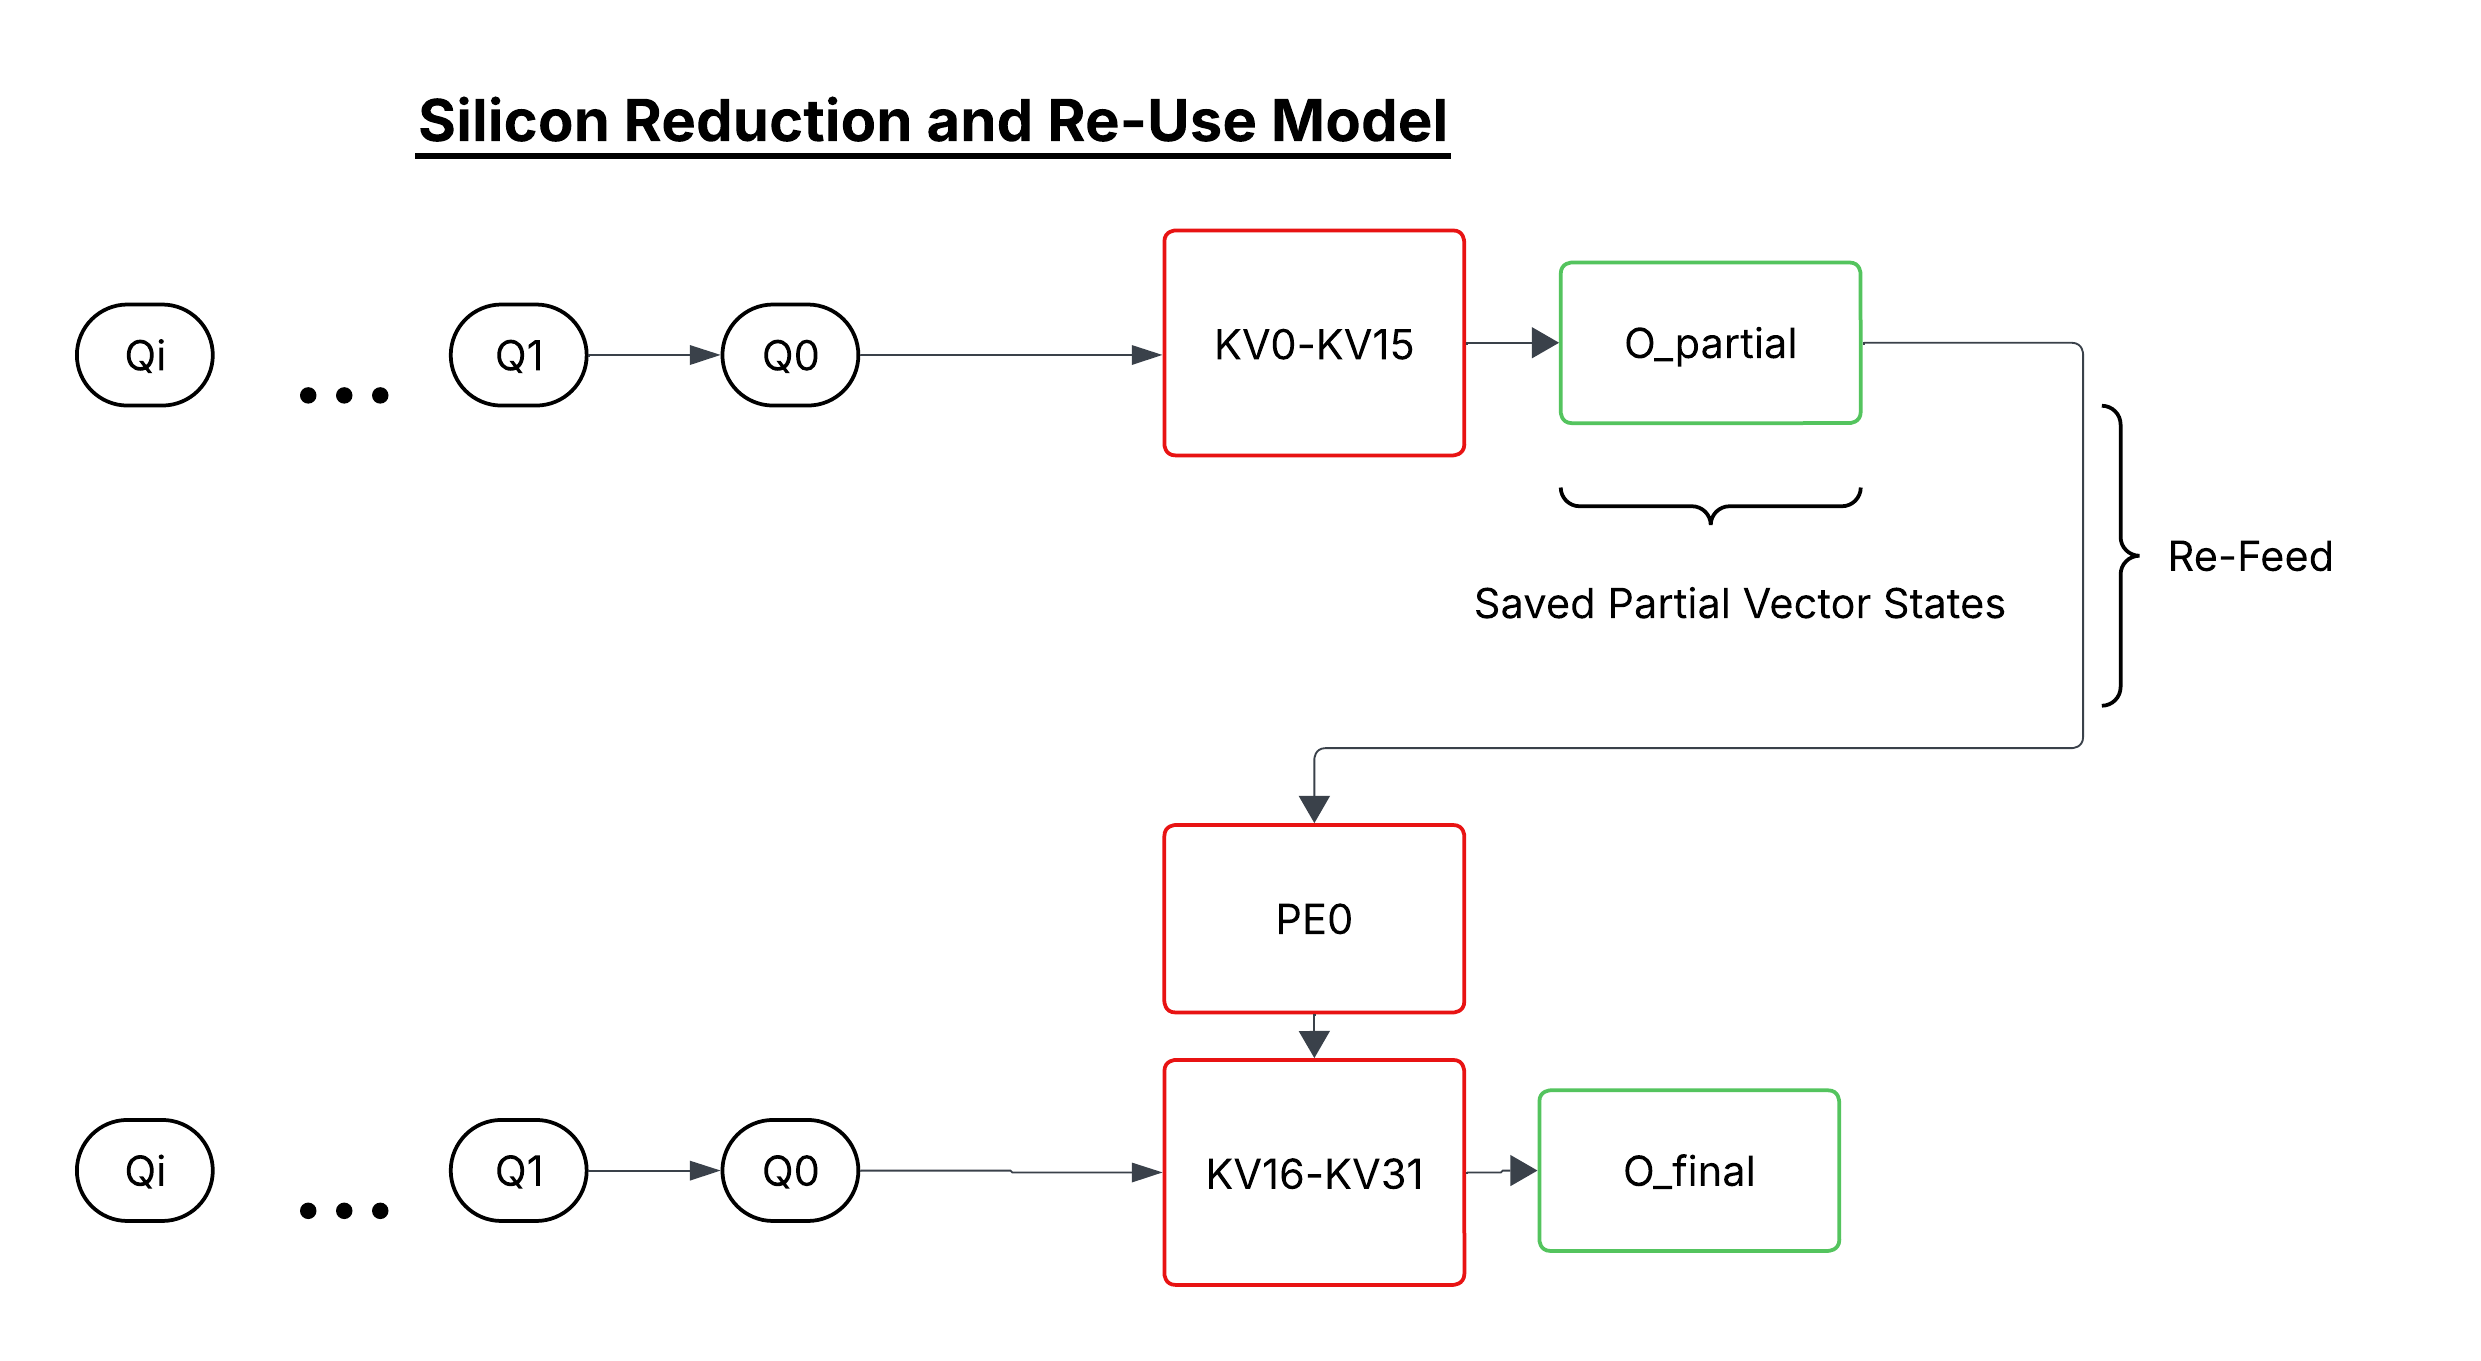
\includegraphics[width=0.82\textwidth]{ReuseModel.png}
    \caption{\textbf{Silicon Reduction and Re-Use Model (\(P = 2\) passes).}
    Pass~1: the query stream attends over the first KV slice (\texttt{KV0--KV15}),
    producing a partial softmax state \texttt{O\_partial} that is saved.
    Pass~2: the same query re-enters and attends over the second slice
    (\texttt{KV16--KV31}); the saved partial state is re-injected via \texttt{PE0}
    so the online softmax continues from the correct running maximum and denominator.
    \texttt{O\_final} is the correctly normalised output over all \(T\) tokens.
    The array uses half the columns (and half the SRAM) of a single-pass design
    at the cost of running each decode token twice.}
    \label{fig:reuse_model}
\end{figure}

\textbf{Silicon reduction and the latency trade-off.}
The re-use model applies to both prefill and decode.
In either phase, using \(P\) passes over a \(T/P\)-column
array instead of one pass over a \(T\)-column array reduces
PE count and SRAM by \(P\times\):

\[
\text{columns} = T / P, \qquad
\text{SRAM\_required} = \frac{2 \cdot T \cdot d \cdot \text{bpe}}{P}
\]

The cost is \textbf{latency}, not DRAM.
Each pass requires the query stream to traverse the array
a second time, and at each pass boundary the partial softmax
state \((m, l, O)\) must be written to a register and
re-injected via \texttt{PE0} at the start of the next pass.
This save-and-reinject overhead is small --- 258 bytes at
FP16 --- but the \(P\times\) pipeline repetition is a real
latency multiplier for both prefill and decode.
There is no DRAM penalty: the KV slices are already resident
on-chip and no additional DRAM traffic is incurred by
the re-use itself.

\begin{center}
\begin{tabular}{lrrll}
\toprule
Passes \(P\) & Columns & On-chip SRAM & Cycle cost & Applies to \\
\midrule
1 & \(T\)     & 128\,MB & \(1\times\) & prefill + decode \\
2 & \(T/2\)   &  64\,MB & \(2\times\) + reinject & prefill + decode \\
4 & \(T/4\)   &  32\,MB & \(4\times\) + reinject & prefill + decode \\
8 & \(T/8\)   &  16\,MB & \(8\times\) + reinject & prefill + decode \\
\bottomrule
\end{tabular}
\end{center}

\textbf{Why this is worth building.}
The primary value is silicon area reduction, not DRAM savings.
The fundamental scaling problem identified in \S7 is that
PE count and SRAM grow linearly with \(T\): at \(T = 8{,}192\)
the single-pass design requires 524K PEs and 128\,MB SRAM.
With \(P = 4\) passes the same computation fits in a
\(T/4 = 2{,}048\)-column array --- 131K PEs and 32\,MB SRAM
--- which is the validated operating point from the prefill
experiments, requiring only \(4\times\) more cycles per token.
In effect, the re-use model lets the designer trade latency
for chip area at a known, controllable ratio, making the
architecture viable at sequence lengths that would otherwise
be physically impractical.

\textbf{Open questions for future validation.}
\begin{itemize}[noitemsep]
    \item SCALE-Sim cycle validation of a single-pass decode step
          (currently divergent due to pipeline drain, as noted in \S\ref{sec:methodology}).
    \item Extending the analytical pipeline model to multi-pass decode,
          including the inter-pass softmax merge cost.
    \item Determining the optimal \(P\) that balances SRAM budget
          against acceptable decode latency for the target workload.
\end{itemize}

% ============================================================
\section{References}

\printbibliography[heading=none]

\end{document}
